\documentclass[9pt]{sigplanconf}
\usepackage{amsmath}
\usepackage{algorithm}
%\usepackage{algorithmic}
\usepackage[vlined,ruled,algo2e,resetcount,linesnumbered]{algorithm2e}
\usepackage{listings}
\usepackage{color}
\usepackage{bm}
\usepackage{pbox}
\usepackage{multirow}
\usepackage{tikz}
\usepackage{multirow}
\usepackage{amsmath}
\usepackage{amsfonts, amssymb}
\usepackage[normalem]{ulem}
\usepackage{color}
\usepackage{epstopdf}


\setcounter{tocdepth}{3}
\usepackage{graphicx}
\usepackage{listings}
\usepackage{multirow}
\usepackage{rotating}
\usepackage{multicol}
\usepackage{url}
\usepackage{color,verbatim,mathabx}
\usepackage{tikz}
\usepackage{setspace}
\usepackage{relsize}
\usepackage{pgfplots}
\usetikzlibrary{automata}
\usetikzlibrary{calc}
\usetikzlibrary{positioning}
\usetikzlibrary{shapes}
\usetikzlibrary{arrows}
\usepgflibrary{arrows}
\usepackage{algorithm}
\usepackage{algorithmic}
\usepackage[vlined,ruled,algo2e,resetcount]{algorithm2e}
\usepackage{tikz}
\setcounter{tocdepth}{3}
\usepackage{graphicx}

\usepackage{url}
\urldef{\mailsa}\path|{alfred.hofmann, ursula.barth, ingrid.haas, frank.holzwarth,|
\urldef{\mailsb}\path|anna.kramer, leonie.kunz, christine.reiss, nicole.sator,|
\urldef{\mailsc}\path|erika.siebert-cole, peter.strasser, lncs}@springer.com|

\usepackage{xcolor, xspace}
\usepackage{listings}
\usepackage{bm}

\definecolor{pink}  {rgb}{0.67, 0.05, 0.57} % keywords
\definecolor{red}   {rgb}{0.87, 0.20, 0.00} % strings
\definecolor{green} {rgb}{0.00, 0.47, 0.00} % comments
\definecolor{violet}{rgb}{0.41, 0.12, 0.61} % classes
%\definecolor{blue}  {rgb}{0.21, 0.00, 0.44} % functions
\definecolor{brown} {rgb}{0.39, 0.22, 0.13} % brown

\definecolor{Brown}{cmyk}{0,0.81,1,0.60}
\definecolor{OliveGreen}{cmyk}{0.64,0,0.95,0.40}
\definecolor{CadetBlue}{cmyk}{0.62,0.57,0.23,0}
\definecolor{lightlightgray}{gray}{0.9}


\newcommand{\locVar}{\mathbb{L}\xspace}
\newcommand{\globVar}{\mathbb{G}\xspace}
\newcommand{\heapVar}{\mathbb{O}\xspace}

\newcommand{\ptr}{{\sf Ptr}}
\newcommand{\ptrset}{{\sf PtrSet}}
\newcommand{\cond}{\mathcal{C}\xspace}
\newcommand{\locReg}{\mathcal{L}\xspace}
\newcommand{\nonlocReg}{\mathcal{N}\xspace}
\newcommand{\Regs}{\Omega \xspace}
\newcommand{\reg}{R}
\newcommand{\CSU}{\mathcal{U}\xspace}
\newcommand{\CSD}{\mathcal{D}\xspace}
\newcommand{\mo}{\delta}
\newcommand{\re}{\theta}
\newcommand{\FI}{\mathcal{I}}
\newcommand{\FO}{\mathcal{O}}
\newcommand{\PTG}{\mathcal{G}}
\newcommand{\Unfoldproc}{\mathcal{E}}
\newcommand{\Mapcs}{\Gamma}
\newcommand{\Mapproc}{\digamma}
\newcommand{\hindent}{\hspace{27mm}}
\newcommand{\true}{\mbox{\sf true}\xspace}
\newcommand{\false}{\mbox{\sf false}\xspace}
\renewcommand{\emptyset}{\varnothing}

\newcommand{\cxtcond}{\mbox{\sf false}\xspace}
\newcommand{\patcond}{\mbox{\sf false}\xspace}
\newcommand{\ComPair}{\mbox{\sf ComPair}}
\newcommand{\level}{\mathcal{L}}

%\newcommand{\fs}{\footnotesize}
\newcommand{\fs}{\fontsize{8}{9}\selectfont}
\renewcommand{\footnotesize}{\fs}
\newcommand{\script}{\fontsize{5}{6}\selectfont}
\newcommand{\smallsize}{\fontsize{7.8}{9}\selectfont}
\newcommand{\verysmall}{\fontsize{5.8}{6.8}\selectfont}
\newcommand{\subfigfont}{\fontsize{10}{10}\selectfont}
\newcommand{\rulefont}{\fontsize{10}{15}\selectfont}
\newcommand{\eqnsubfont}{\fontsize{6}{6}\selectfont}

\newcommand{\cupunion}{\ \cup\hspace{-0.8mm}=}

\newcommand{\alias}{{\sf AS}}
\newcommand{\pts}[1]{\textsf{Ptr}\lfloor{#1}\rceil}
\newcommand{\stmt}[1]{\langle{#1} \rangle}
\newcommand{\trans}[1]{\mathcal{T}{(#1)}}
\newcommand{\transcs}{\mathcal{T}}
\newcommand{\meet}[1]{\Upsilon{(#1)}}
\newcommand{\ptsinf}{\rhd}
\newcommand{\transinf}{\diamond}
\newcommand{\tfinf}{;}
\newcommand{\evaltfinf}{\odot}
\newcommand{\applytfinf}{\Join}
\newcommand{\regapplytfinf}{\xspace \boxdot_{\textsf{call}_k} \xspace}
\newcommand{\modrefinf}{:\xspace}
\newcommand{\ruleindent}{\hspace{5mm}}
\newcommand{\modset}{\mathcal{D}}
\newcommand{\refset}{\mathcal{U}}
\newcommand{\vect}[1]{\widehat{#1}}
\newcommand{\curana}[1]{\Vert{#1}\Vert}
\newcommand{\parorder}{\sqsupset \xspace}
\newcommand{\parordereq}{\circeq \xspace}
\newcommand{\dominate}{\preccurlyeq \xspace}
\newcommand{\regset}{\mathcal{S}}
\newcommand{\intermap}{\mathcal{M}}
\newcommand{\eval}{\textsf{Eval}\xspace}
\newcommand{\embf}[1]{\textbf{\emph{#1}}}

\newtheorem{example}{Example}
\newtheorem{definition}{Definition}
\newtheorem{lemma}{Lemma}
\newtheorem{theorem}{Theorem}
\newtheorem{property}{Property}

\newcommand*{\longhookleftarrow}{\ensuremath{\leftarrow\joinrel\relbar\joinrel\rhook}}
\newcommand*{\longhookrightarrow}{\ensuremath{\lhook\joinrel\relbar\joinrel\relbar\joinrel\relbar\joinrel\rightarrow}}

\newcommand{\stackleftarrow}[1]{\stackrel{#1}{\hookleftarrow}}
\newcommand{\stackeq}[1]{\stackrel{#1}{=}}
\newcommand{\stackcupunion}[1]{\ \cup\hspace{-0.8mm}\stackeq{#1}}

\newcommand{\ruledef}[3]{ \rulename{#1} & $\frac{\begin{array}[c]{c}#2\end{array}}{\begin{array}[c]{c}#3\end{array}}$}
\newcommand{\ruledefX}[2]{ \rulename{#1} & $\begin{array}[c]{c}#2\end{array}$}
\newcommand{\rulename}[1]{{\small\texttt{[\MakeUppercase{#1}]}}}

\newcommand*\circled[1]{\tikz[baseline=(char.base)]{
            \node[shape=circle,draw,inner sep=0pt] (char) {#1};}}

% Code from Christian Feuersänger
% http://tex.stackexchange.com/questions/54794/using-a-pgfplots-style-legend-in-a-plain-old-tikzpicture#54834

% argument #1: any options
\newenvironment{customlegend}[1][]{%
    \begingroup
    % inits/clears the lists (which might be populated from previous
    % axes):
    \csname pgfplots@init@cleared@structures\endcsname
    \pgfplotsset{#1}%
}{%
    % draws the legend:
    \csname pgfplots@createlegend\endcsname
    \endgroup
}%

% makes \addlegendimage available (typically only available within an
% axis environment):
\def\addlegendimage{\csname pgfplots@addlegendimage\endcsname}
%%--------------------------------


\begin{document}

\conferenceinfo{ISMM '13}{June 20-21, Seattle Washington}
\copyrightyear{2013}
\copyrightdata{[to be supplied]}



%\titlebanner{banner above paper title}        % These are ignored unless
\preprintfooter{Correlated Aliasing Strong Updates}   % 'preprint' option specified.

\title{Correlated Aliasing Strong Updates}
%\subtitle{Subtitle Text, if any}

\authorinfo{Name1}
           {Affiliation1}
           {Email1}
\authorinfo{Name2\and Name3}
           {Affiliation2/3}
           {Email2/3}

\maketitle


%\newcommand{\ptrset}[1]{PtrSet(#1)}
\newcommand{\ptrmap}[1]{PtrMap(#1)}


\lstdefinelanguage{Objective-C 2.0}[Objective]{C} {
    morekeywords={id, Class, SEL, IMP, BOOL, nil, Nil, NO, YES,
                  oneway, in, out, inout, bycopy, byref,
                  self, super, _cmd,
                  @required, @optional,
                  @try, @throw, @catch, @finally,
                  @synchronized, @property, @snythesize, @dynamic},
    moredelim=[s][color{red}]{@"}{"},
    moredelim=[s][color{red}]{<}{>}
}

\lstdefinestyle{Xcode} {
    language        = Objective-C 2.0,
    basicstyle      = \smallsize \ttfamily,
    identifierstyle = \color{black},
    commentstyle    = \color{green},
    keywordstyle    = \color{pink},
    stringstyle     = \color{green},
    directivestyle  = \color{brown},
    extendedchars   = true,
    tabsize         = 4,
    showspaces      = false,
    showstringspaces = false,
    breakautoindent = true,
    flexiblecolumns = true,
    keepspaces      = true,
    stepnumber      = 0,
    xleftmargin     = 0pt
    }

\lstset{
    style = Xcode,
%    caption=lstname,
    breaklines=false,
    numbers=left, numberstyle=\fs,
%    frame=single,
    emph = {PerlMem_realloc,malloc,free,realloc, remove_duplicate, strdup,calloc,gl_alloc_texture_object},
    emphstyle = \color{red}\underbar
}



\begin{abstract}
Strong updates are to enable flow sensitive analysis to kill old pointer information when a variable is assigned new information. Strong update for top-level pointers in C are trivial in SSA form. For indirect strong updates, a.k.a, strong update for address-taken variables, previous approaches consider singleton, which means information can only be killed when points-to set of the dereferenced pointer containing at most one memory object. In this paper, we propose a novel approach to explore correlated aliasing on \emph{memory regions} for strong updates. (\textbf{NEEDS A REWRITE})

%\keywords{Points-to analysis; Strong updates; Flow-Sensitivity}
\end{abstract}

\category{CR-number}{subcategory}{third-level}

%\terms term1, term2

\keywords
keyword1, keyword2



\section{Introduction}
Pointer analysis is to statically approximate runtime value of a pointer in memory. It is a key analysis for both compiler optimizations \cite{das2001estimating,lhotk,hind2000pointer} and memory-related software error detection \cite{Livshits03, xie2007saturn,le2008marple,dillig2011precise}. Analysis with high precision can give more opportunities for aggressive optimizations and accurate bug detection. 
As clients increasingly require high precision, there has been quite a few recent advanced techniques for more precise pointer analysis \cite{kahlon2008bootstrap,strongupdate,hardekopfflow,hardekopf2009semi, yu2010level,li2011boosting,De:2012}.
Strong updates are the most important feature in flow sensitive pointer analysis for precision improvement \cite{hardekopf2009semi,hardekopfflow,strongupdate,li2011boosting}. It can also be used to incorporate with context sensitive analysis to achieve further accuracy \cite{dillig2011precise,De:2012}. 
Strong updates enable the analysis to kill the old points-to information of a memory location  when this location is assigned a new value. In contrast, weak updates keep the old information unchanged while adding new values. 

%Strong update aids the analysis to be more accurate by updating the analysis results. 
An abstract location \emph{v} at a program statement can be strongly updated if and only if \emph{v} refers to at most one concrete memory location. 
It is trivial to enable strong updates for \emph{top-level} pointers on SSA (Static Single Assignment) form \cite{strongupdate,hardekopfflow,yu2010level,hardekopf2009semi}. Because of the nature that each variable can only have one definition on SSA, \emph{top-level} pointers whose address are not taken can be directly renamed just like scalars. As a result, a pointer defined at different program points can be easily distinguished with unique names. However, 
the difficulty lies at analyzing \emph{address-taken} pointers, given an address-taken pointer \emph{v} pointed by \emph{x}, accordingly, \emph{v} can be indirectly accessed by \emph{x}, 
strong updates for variable \emph{v} at a \emph{store} statement \emph{*x=y} can not be fully processed until the points-to relation of \emph{x} is computed. Previous algorithms \cite{strongupdate,hardekopfflow,hardekopf2009semi, yu2010level,li2011boosting,wilson1995efficient,emami1994context} handle \emph{indirect} strong updates at \emph{store} statements in terms of \emph{singleton}, provided that the points-to set of a dereferenced pointer contains at most one concrete memory location. More specifically, the old value of \emph{v} can be killed, and updated to the value of \emph{y} after the statement if and only if \emph{*x} refers to the unique location \emph{v} in any execution paths. 

%SSA form are commonly used in existing compilers like GCC/LLVM/Open64, in SSA form, every variable only has a unique definition at a certain program point. 
%considers the points-to set of a dereferenced pointer contains at most one memory locations to 

\begin{figure}[tp]
\centering
\hspace*{0mm}
\begin{tabular}{ |@{\hspace{0mm}} c @{\hspace{0mm}}@{\hspace{0mm}} c @{\hspace{-2mm}}| }\hline


\begin{tabular}{  @{\hspace{-1mm}}l@{\hspace{0.5mm}}|  }
\textcolor{pink}{void} \textsf{main}()\{\\
\textcolor{pink}{int} **$x$,*$y$,*$z$,*$a$,*$b$,*$p$,$c$,$m$,$n;$\\
\hspace{2.4mm}   $y$ = $\&c;$ $a$ =$\&m;$ $b$=$\&n;$\\
\begin{tabular}{r@{\hspace{1mm}}l@{\hspace{1mm}}l}
\hspace{1mm}\textcolor{pink}{if}(*) \{ $x$ &=& $\&a;$ \}\\
\hspace{1mm}\textcolor{pink}{else}\hspace{0.65mm}  \{ $x$ &=& $\&b;$ \}\\
\hspace{5.6mm}     \circled{*$x$} &=& $y;$\\
\hspace{6.4mm}     $z$ &=& $x;$\\
\hspace{6.4mm}     $p$ &=& \circled{*$z$}; \\
\end{tabular}
\\
\}
%\hspace{2mm}\textcolor{green}{// p$\dashrightarrow$m, p$\dashrightarrow$n, p$\longrightarrow$c}\\
\end{tabular}

&

\begin{tabular}{  @{\hspace{0mm}}l  }
\textcolor{pink}{void} \textsf{main}()\{\\
\textcolor{pink}{int} **$x$,*$y$,*$r$,*$a$,*$b$,*$p$,$m,c,d;$\\
\hspace{2.4mm}   $x$ = $\&y;$ $y$ = $\&m;$ $r$ = $\&m;$\\
\hspace{2.4mm}	$a$ =$\&c;$ $b$ = $\&d;$ \\
\begin{tabular}{r@{\hspace{1mm}}l@{\hspace{1mm}}l}
\textcolor{pink}{if}(*)   \{ \hspace{2.2mm}$x$ &=& $\&r;$ \}\\
\textcolor{pink}{if}(*) \{ \circled{*$x$}  &=& $a;$ \}\\
\textcolor{pink}{else}\hspace{1.25mm}  \{ \circled{*$x$} &=& $b;$ \}\\
     $p$ &=& \circled{*$x$};\\
\end{tabular}
\\
\}
%\hspace{2mm}\textcolor{green}{// p$\dashrightarrow$m, p$\dashrightarrow$n, p$\longrightarrow$c}\\
\end{tabular}

\\\hline

\begin{tabular}{l@{\hspace{6mm}}|}
\fs $p\hspace{-0.4mm} \rightarrow\hspace{-0.5mm}c$ \quad $p\hspace{-1mm}\dashrightarrow\hspace{-0.5mm}m$ \quad $p\hspace{-1mm}\dashrightarrow\hspace{-0.5mm}n$ \\ 
\end{tabular}
&
\begin{tabular}{l}
\fs \quad $p\hspace{-0.4mm} \rightarrow\hspace{-0.5mm}c$ \quad $p\hspace{-0.4mm} \rightarrow\hspace{-0.5mm}d$ \quad $p\hspace{-1mm}\dashrightarrow\hspace{-0.5mm}m$ \\
\end{tabular}
\\ \hline


\begin{tabular}{  @{\hspace{0.5mm}}l@{\hspace{1mm}}|@{\hspace{-2mm}}   }
\hspace{-4mm}(a) \fs intra correlated aliases (*x,*z)
\end{tabular}
& 
\begin{tabular}{  @{\hspace{-2mm}}l@{\hspace{-2mm}}  }
(b) \fs intra correlated aliases (*x,*x)
\end{tabular}

\\ \hline

\begin{tabular}{  l  }
\textcolor{pink}{int} $g$, $m$, $n;$\\
\textcolor{pink}{void} \textsf{main}()\{\\
\hspace{0mm}\textcolor{pink}{int} **$w$,** $v$,**$r$,*$a$,*$b$, *$t$, *$s;$\\
\hspace{0mm}  $w$ = $\&a;$ $v$ = $\&b;$ $r$ = $\&t;$\\
 \hspace{0mm}    $a$ = $s$ = $\&m;$ $b$ = $t$ = $\&n;$\\
 \hspace{3.6mm}     foo(w, w, r) \ \textcolor{green}{// \emph{SU for t}}\\
 \hspace{4mm}\textcolor{pink}{if}(*) \{ $r$ = $\&s;$ \} \\
 \hspace{3.4mm}     foo(v, v, r) \ \textcolor{green}{//\emph{WU for t, s}} \\
\}
%\hspace{2mm}\textcolor{green}{// p$\dashrightarrow$m, p$\dashrightarrow$n, p$\longrightarrow$c}\\
\end{tabular}

&
\hspace{-6mm}
\begin{tabular}{  l  }
\\
 \hspace{1.4mm}  \textcolor{pink}{void} \textsf{foo}(\textcolor{pink}{int}** x, \textcolor{pink}{int}** y, \textcolor{pink}{int}** z)\{\\
 \hspace{5.6mm} \textcolor{pink}{int} *$p$, *$q;$\\

 \begin{tabular}{r@{\hspace{1mm}}l@{\hspace{1mm}}l}
 \hspace{4.6mm}     $q$ &=& $\&g$; \\
 \hspace{4.6mm}     \circled{*$x$} &=& $q;$\\
 \hspace{6.4mm}     $p$ &=& \circled{*$y$}; \\
 \hspace{6.4mm}     $*z$ &=& $p;$
 \end{tabular}
\\
 \hspace{1.4mm}     \}
%\hspace{2mm}\textcolor{green}{// p$\dashrightarrow$m, p$\dashrightarrow$n, p$\longrightarrow$c}\\
\end{tabular}
\\\hline

\multicolumn{2}{|c|}{
\begin{tabular}{@{\hspace{20mm}}l @{\hspace{15mm}}}
\fs \quad $p\hspace{-0.4mm} \rightarrow\hspace{-0.5mm}g$ \quad $p\hspace{-0.4mm} \dashrightarrow\hspace{-0.5mm}m$ \quad $p\hspace{-1mm}\dashrightarrow\hspace{-0.5mm}n$ 

\end{tabular}
}

\\ \hline

\multicolumn{2}{|c|}{
(c) \fs inter correlated aliases (*x,*y)
}
\\ \hline


\end{tabular}
\caption{Strong updates with correlated aliases. Spurious points-to relations are labeled with dashed arrows ($\dashrightarrow$) according to \emph{Singleton} based strong updates algorithm. \label{fig:motex}}
\end{figure}



\emph{Singleton} algorithm performs weak updates whenever a dereferenced pointer contains more than one concrete object. An example is shown in Figure~\ref{fig:motex}(a), \emph{x} points to two objects \emph{a} and \emph{b} from different branches at the entry of statement \emph{*x=y}. Thus, \emph{a} and \emph{b} can only be weakly updated after analyzing the fourth statement, the old points-to target \emph{m} is kept while adding the new value \emph{c} into the points-to set of \emph{a}. Likewise, both \emph{n} and \emph{c} are pointed by \emph{b}. \emph{Singleton} algorithm considers indirect strong updates at a \emph{store} statement independently, while overlooks its correlations with another pointer dereference (e.g. dereference at \emph{load} statements), which leads to weakly updated information at a \emph{store} to be propagated unconditionally to any aliased expression. For example, Figure~\ref{fig:motex}(a) shows that weakly updated points-to value of \emph{a} and \emph{b} at the fourth statement are assigned to pointer pointer \emph{p} when handling \emph{load} operation at statement \emph{p=*z}. However, in real runtime execution scenarios, two aliases \emph{*x} and \emph{*z} always refer to exactly the same memory location in any program path. Therefore, strong updates occurs when considering the value flows between these two aliased expressions. Consequently, \emph{m} and \emph{n} in the points-to set of \emph{a} and \emph{b} are blocked for propagation from \emph{*x} to \emph{*z}, and only points-to target \emph{c} of \emph{y} can flow through this pair of aliases to \emph{p}. (\textcolor{red}{Similarly for Figure~\ref{fig:motex}(b)(c)}) 

Comparing to \emph{Singleton} based algorithms which focus only on \emph{store} statements for \emph{indirect} strong updates, our approach performs strong updates beyond single memory location limitation by looking at a pair of aliased expressions (e.g. $\langle x, *y \rangle$, $\langle *x, *y \rangle$, $\langle *x, *x \rangle$ ). The key insight behind our approach is to consider points-to propagation between a \emph{correlated aliases} pair instead of counting the number of memory locations at a pointer dereference alone. Strongly updated information can flow from a definition into its uses between \emph{correlated aliases}. More strong updates can be obtained comparing with conventional \emph{Singleton} approach.
%determine two aliased expressions which are correlated under same program paths, then the expression itself can propagating strongly updated points-to information from definition of the aliases to use of another aliases no matter how many memory location it contains. 

Capturing correlations between a pair of aliases is challenging. 
First, points-to and aliasing analysis are cyclic dependent. On the one hand, for the sake of computing points-to relations by strong updates, correlated aliasing needs to be figured out. On the other hand, in order to decide whether a pair of aliased expressions are correlated (e.g.$\langle x, *y \rangle$), the points-to value of a dereferenced pointer \emph{y} requires to be computed first. The naive approach is to use a cheap/imprecise analysis \cite{andersen1994program,steensgaard1996points} to distinguish aliases before strong updates. However, it might be too conservative to generate overwhelming imprecise aliases for correlation analysis. Ideally, correlated aliasing strong updates should be done at the same time when performing points-to resolution. Our way is to use a level-wised approach to partition pointer-related expressions into different levels, higher levels are analyzed prior to lower levels. With well-define processing order, earlier analysis can be used to bootstrap later phase analysis to generate precise results. 

In addition, the precision of aliasing analysis is impacted by diverse factors (e.g. flow, context sensitivity), another challenge is how to effectively identify various correlation patterns when taking these multidimensional factors into account. By making use of flow sensitive analysis, the correlation connection between \emph{*x} and \emph{*z} is captured by assignment at statement \emph{z=x} in Figure~\ref{fig:motex}(a).  However, correlations between two aliases are not limited to flow sensitivity. In practice, many aliases are correlated when considering their calling contexts and control-flow paths. Essentially, efficient and accurate algorithms which can easily leverage recent advanced analysis are crucial and attractive. 

The following are the key contributions in this paper:
\begin{itemize}
\item A novel strong updates approach by considering the correlation between a pair of aliases for generating more precise strong updates than \emph{Singleton} based algorithms
\item Correlated aliasing analysis by considering flow, context and program paths information.
\item A new level-wised memory region-based sparse analysis.
\item We evaluate our \emph{correlated aliasing} strong updates by comparing with \emph{singleton} based algorithms and various correlation factors (e.g. context-, path-) with XXX benchmarks and XXX open source programs, our approach can have XXX more strong updates while keep the compatible analysis time XXX with state-of-art FSCS points-to analysis algorithms.
\end{itemize}



%Points-to set of the dereferenced pointer containing at most one memory object
%Points-to set of lower level pointers can be computed after analyzing high level pointers.



\section{Language And Preliminaries \label{sec:lang}}
%\section{Analysis Overview}
A simple C-like language abstract syntax is given in Figure~\ref{fig:simplelang} for our analysis.
In the canonical form, a statement in the CFG of an input program is one of the following:
(1) an assignment of the form, $p=\&q$ (\texttt{address}), $p=q$ (\texttt{copy}), $*p=q$ (\texttt{store}) or $p=*q$ 
(\texttt{load}), where $p$ and $q$ are local, global or heap variables, (2)
 a call $v =$ \textsf{call}$_k$$(p,\dots,q)$ at callsite $k$,
where $v$, $p,\dots,q$ are all local variables,
and (3)
a return statement, \textsf{return}$_t(v)$ at return site $t$, where $v$ is a local variable. 
(4) a two-way branch (i.e., an if-statement), which is missing in Figure~\ref{fig:simplelang} will be considered after translating the program into SSA representation in Figure~\ref{fig:ssalang}.

Generally, pointer analysis with strong updates applies iterative data-flow approach for resolution. Each statement \emph{s} on the control flow graph (CFG) is analyzed with input points-to relations propagated from predecessors of \emph{s} and outgoing points-to value are generated after analyzing \emph{s}. Accordingly, the output points-to relations are then propagated to successors of \emph{s} along the CFG for further computation. The propagation and resolution terminate until a fixed point is reached. However, iterative data-flow analysis is costly, as it propagates pointer information blindly from each node in the CFG to its successors without knowing if the information will be used there or not, which incurs huge analysis overhead and memory consumption especially when analyzing large programs \cite{hardekopf2009semi}. On the contrary, a sparse analysis \cite{hardekopf2009semi,sui2011spas,oh2012design,yu2010level,hardekopfflow,li2011boosting}  propagates the pointer information from defs of the variables directly to their uses along their def-use chains, but, unfortunately, the def-use information can only be computed using the pointer information. To break the cycle, a sparse pointer analysis typically proceeds in stages: def-use chains are initially approximated based on some fast pointer analysis and then refined in a sparse manner. 


\begin{figure}[t]
\centering
\begin{tabular}{l@{\hspace{3mm}}ll@{\hspace{3mm}}l}
Local	&	\emph{l}		\\
Global	&	\emph{g}		\\
Heap		&	\emph{o}		\\
Location		&	$v,p,q$ 	& $::= $  & $ l \mid g \mid o$\\
Stmt & \emph{s} & $::=$ & $p = \&q \mid p = q$	 $\mid p = *q \mid p = q$\\
		  &			 &		 & $\mid v = \textsf{call}_k(p,\dots q)$ $\mid \textsf{return}_t(v)$\\
%		  &			 &		 & $\mid s_1;s_2$ $\mid$ \textsf{if}(*) $s_1$ \textsf{else} $s_2$ $\mid$ \textsf{while}(*) $s$\\
%Condition & \emph{c} & $::= $ & \emph{f}$\cup \{s\} \mid \emptyset$ \\
%Condition	& $C,M$ & $::= $ & $true \mid false \mid \neg C \mid C_1 \vee C_2 \mid C_1 \wedge C_2$\\
Procedure & \emph{f} & $::= $ & \emph{f}$\cup \{s\} \mid \emptyset$ \\
%Region & $\reg$ & $::=$ & $\{v\} \mid \reg \cup \reg \mid \emptyset $	\\
%May-Use & $\re$ & $::=$ & $\{\mu(v_i)\} \mid \re \cup \re \mid \emptyset  $	\\
%May-Def & $\mo$ & $::=$ & $\{v_i = \chi(v_j)\} \mid \mo \cup \mo \mid \emptyset $	\\
%Sel-Label & $\Phi$ & $::=$ & $\emptyset \mid \{r\} \mid l \cup l$	\\
%Procedure & \emph{f} & $::=$ & $\emptyset \mid \{v\} \mid r \cup r$	\\


\end{tabular}
\caption{Abstract syntax of programs.
\label{fig:simplelang}}
\end{figure}

%As sparse analysis now is the mainstream for scalable flow sensitive points-to analysis.
%Due to the nature that each variable has unique definition on SSA and its built-in def-use chains, A sparse pointer analysis usually performs on SSA form  \cite{hardekopf2009semi,sui2011spas,yu2010level,hardekopfflow,li2011boosting}. 
Sparse points-to analysis on SSA form can significantly speed up analysis for large programs \cite{hardekopf2009semi,sui2011spas,yu2010level,hardekopfflow,li2011boosting}. However, it can not simply be adopted for our correlated aliasing strong updates. Several challenges need to be overcome: different from eariler sparse points-to analysis \cite{hardekopf2009semi,yu2010level,hardekopfflow} which only calculate points-to result of a variable, our approach needs to analyze correlations between two aliased expressions simultaneously when doing pointer resolution. Therefore, both pointers (e.g. p) and dereference expressions (e.g. *p) are required to be sparsely represented on SSA. During our full-sparse SSA construction, a memory region $R$ is introduced (Figure~\ref{fig:ssalang}) to stands for an expression (e.g. $p_i,*p_i$), which represents a set of
memory locations. For brevity, given a single variable expression $p$, $R(p)$ and 
$p$ are used interchangeably to stand for the region. Statements are transformed into region-based statements as shown in Figure~\ref{fig:ssalang}. Unlike previous sparse SSA form \cite{yu2010level, hardekopfflow}, we put regions instead of individual variables on SSA for renaming. Each region is defined exactly once in the program, distinct definitions of a region are distinctly versioned.  

There are many ways for creating a memory region, in one extreme, every expression like \emph{*p} in the program can be treated as a region. However, \emph{p} might be redefined to different versions like $p_i$ and $p_j$ at distinct program points on SSA, thereby referring \emph{*p$_i$} and \emph{*p$_j$} to the same memory region is imprecise. In another extreme, in order to create an exact region for \emph{*p}, pointer \emph{p} needs to be SSA renamed and fully solved first before region creation of \emph{*p}. We arrange a well-defined processing order for analyzing different expressions so as to create precise regions for incrementally building full-sparse SSA form (Section~\ref{sec:su}).

%indirectly read (MAY-USE) at a load or indirectly modified (MAY-DEF) at a store. 
%Sparse analysis can significant speed up the analysis, However, only sparsity is not enough for effectively capture the correlated aliasing relations. 
%recent works pay great attention to flow sensitivity on SSA form. As strong update for top level are naturally supported.
%Escape order based or level-wised analysis not only can bootstrap later phase analysis but can also reduce the points-to propagation.

During construction of SSA for all regions, three new types of operators $\Phi$, $\mu$, and $\chi$ are introduced following \cite{chow1996effective}. 
%The $\Phi$ functions are added at join points as is standard. 
At a join point in the control-flow graph (CFG)
of the program, all versions of the same region reaching the point are combined using  a $\Phi$ function, producing a new version for the region. Different from \cite{chow1996effective}, \textsf{address}, \textsf{copy}, \textsf{stores} and \textsf{loads} (Figure~\ref{fig:simplelang}) are all unified into a simple \emph{region copy} statement  $\stmt{R \stackleftarrow{\fs s} R^\bullet}_\mo$ (Figure~\ref{fig:ssalang}).    
Only $\chi$ functions instead of $\mu$ is annotated for each \emph{region copy} statement $s$.  May-Def list $\mo$, which is a list of $\chi$ functions, such that every  $R'\!=\!\chi(R')$ denotes a region $R'$ is aliased with $R$ and may be potentially defined at $s$. $\chi$ function is treated as a definition, suppose $R'\!=\!\chi(R')$ becomes $R'_m\!=\!\chi(R'_n)$ after SSA conversion.
$R'_m$ can be strongly updated if $R'$ \emph{must alias} with $R$, In this case, $R'_m$ receives whatever $R^\bullet$ points to and the information in $R'_n$ is ignored. Otherwise, $R'_m$ must incorporate the pointer information from both $R'_n$ and $R^\bullet$.
%Each load $p=*q$ is annotated with  a May-Use list, $\re$, which is a list of $\mu$ functions, such that every $\mu(R)$ denotes a region $R$ that may be potentially read at the load. Similarly, each store $*p=q$ is annotated with a May-Def list, $\mo$, which is a list of $\chi$ functions, such that every $R=\chi(R)$ indicates a region $R$ that may be potentially defined at the store. 
%To understand this asymmetric treatment of $\mu$ and $\chi$, suppose $R\!=\!\chi(R)$ (associated with $*p=q$) becomes $R_m\!=\!\chi(R_n)$ after SSA conversion. If $p$ uniquely points to $R$, which represents a single concrete memory location, then $R_m$ can be strongly updated. In this case, $R_m$ receives whatever $R$ points to and the information in $R_n$ is ignored. Otherwise, $R_m$ must incorporate the pointer information from both $R_n$ and $q$.
May-Use list $\re$, which is a list of $\mu$ functions annotated only at a callsite or return statement $s$, such that every $\mu(R)$ denotes a region $R$ that may be potentially read at $s$.
Every callsite is annotated with a May-Use list $\re$ and a May-Def list $\mo$. Every return statement is annotated with a May-Use list $\re$ to represent the list of regions that may indirectly return to a caller. 

Each $\mu/\chi$ are associated with condition $C$, $P$ and $M$ to specify under which condition the indirect read/modification holds.  $C$ stands for \emph{context condition} represented as Boolean expressions over the set of
points-to relations to be introduced in Section~\ref{sec:inter}. $P$ is a set of intra-procedure \emph{path condition} represented as Boolean expressions encoding the branches in a CFG to be introduced in Section~\ref{sec:intra}. In order to perform strong updates, $M$ is a special \emph{must condition} to represent under which a region in the $\mu/\chi$ must be used/modified (\emph{must alias}). It uses the calling contexts encoded similarly as $C$ when performing inter-procedure analysis (Section~\ref{sec:inter}). For intra-procedure analysis, its value is either \true or \false (Section~\ref{sec:intra}).

%When converted to SSA form using a standard algorithm \cite{chow1996effective,cytron1991efficiently}, each  $\mu(R)$ is treated as a use of $R$ and
%each $R=\chi(R)$ is treated as both a def and use of $R$.

%Once all regions are identified, 
Once indirect defs and uses at loads, stores and
callsites are exposed by adding $\mu$ and $\chi$ 
functions and then the conversion to SSA can take place using
a standard SSA algorithm~\cite{chow1996effective,cytron1991efficiently}. 

%Our incremental SSA construction includes inserting $\mu/\chi$ function and SSA renaming (SSA conversion). SSA renaming is standard after inserting $\mu/\chi$ \cite{chow1996effective,cytron1991efficiently}, thus the algorithm is ignored in the following section, our main task is to determine side-effects at a statements by $\mu/\chi$ function during full-sparse SSA construction.

\begin{figure}[t]
\centering
\begin{tabular}{l@{\hspace{2mm}}ll@{\hspace{1mm}}l}

Region & $\reg,\reg',\reg^\bullet $ & $::=$ & $p \mid *p \mid \&p$	\\
Region& \emph{s} & $::=$ & $\stmt{R \stackleftarrow{\fs s} R^\bullet}_\mo$	\\ 
Based %&			 &		 & $\mid \stmt{p = R(*q)}^\re \mid \stmt{R = R'}_\mo$\\
Stmt		  &			 &		 & $\mid \stmt{R \stackleftarrow{\fs s} \Phi(R,R)}$\\
		  &			 &		 & $\mid \stmt{R \stackleftarrow{\fs s} \textsf{call}_k(R',\dots,R^\bullet)}^\re_\mo$ \\
		  &			 &		 & $\mid \stmt{\textsf{return}_t(R)}^\re$\\
%		  &			 &		 & $\mid s_1;s_2$ $\mid$ \textsf{if}(*) $s_1$ \textsf{else} $s_2$ $\mid$ \textsf{while}(*) $s$\\
%Condition & \emph{c} & $::= $ & \emph{f}$\cup \{s\} \mid \emptyset$ \\
Condition & $C,P,M$ & $::= $ & $true \mid false \mid \neg C$ \\
		  &			 &		 &   $\mid C_1 \vee C_2 \mid C_1 \wedge C_2$\\
%Procedure & \emph{f} & $::= $ & \emph{f}$\cup \{s\} \mid \emptyset$ \\
May-Use & $\re$ & $::=$ & $\{\mu(R,C,P,M)\} \mid \re \cup \re \mid \emptyset  $	\\
May-Def & $\mo$ & $::=$ & $\{R = \chi(R,C,P,M)\} \mid \mo \cup \mo \mid \emptyset $	\\
%Sel-Label & $\Phi$ & $::=$ & $\emptyset \mid \{r\} \mid l \cup l$	\\
%Procedure & \emph{f} & $::=$ & $\emptyset \mid \{v\} \mid r \cup r$	\\


\end{tabular}
\caption{Extended abstract syntax of memory region based representation on full-spasre SSA form (a subscript associated with each region which stands for SSA version is ignored for brevity here).
\label{fig:ssalang}}
\end{figure}


\section{Correlated Aliasing Strong Updates \label{sec:su}}
Two aliased regions are correlated whenever they can be represented by the same memory object along identical program path during runtime.
Aliasing and points-to analysis are cyclic dependent. In order to break the cycle, a pre-analysis is used by Steensgaard algorithm \cite{steensgaard1996points} to bootstrap later phase analysis. Given an unification-based points-to graph with all nodes represented by regions, all predecessors of each node are merged, and finally, make the points-to graph acyclic by collapsing SCCs. The points-to level of a region is its longest length over \{0, . . . , L\} to a sink node. Regions at higher levels are analyzed first so as to provide points-to information for analyzing regions at lower levels.


\begin{definition}
\label{def:order}
Processing Order: given two regions $R'$ and $R$ on SCC-unification points-to graph, $R' \parorder R$ denotes $R'$ is analyzed before $R$, $R' \parordereq R$ stands for $R'$ is analyzed together $R$.
\end{definition}


According to \emph{Processing Order}, our analysis is partitioned into two parts as shown in Figure~\ref{fig:overview}
: incremental SSA construction by inserting $\mu/\chi$ functions to identify correlations and  pointer resolution for strong updates with correlated aliasing constraints. These two parts are processed iteratively by analyzing regions from highest to lowest level.


\begin{definition}
\label{def:ptr}
Points-to Set and Aliasing Set: For a region R, $(v,C,P,M) \in \ptr(R)$ contains a set of tuples representing that $R$ points to location $v$ under context $C$ along path $P$, the points-to must holds under condition $M$. Similarly, $(v,C,P,M) \in \alias(R)$ denotes location $v$ is represented by R under context $C$ along path $P$, $v$ is definitely represented by $R$ if and only if $M$ holds.
\end{definition}

\begin{figure}[t] %  figure placement: here, top, bottom, or page
\centering
\hspace*{-5mm}
\scalebox{0.745}{
	
	%add table and then two sub figure will be one the same line
	
\begin{tikzpicture}[thick]
	\begin{scope}[node distance=8.4mm]

	\node [rectangle,draw=black!50,minimum height=5mm,minimum width=15mm](B_{1}) []{
	\begin{tabular}{c}
	\\
%	Given $e \parorder e'$  $e$ is analyzed before $e'$ \\
	\textbf{\large Pre-Analysis}\\
	\\
	\end{tabular}
	};
				
	\node [node distance=0.1cm](B_{0}) [node distance=4mm,left=of B_{1}]{};
						
	\node [node distance=0.1cm](1) [left=of B_{1}]{};
	
	\node [rectangle,draw=black!50,minimum height=5mm,minimum width=20mm](B_{2}) [right=of B_{1}] {
	\begin{tabular}{c}
	\textbf{\large Incremental}		\\
	\textbf{\large Full-Sparse SSA}	\\
	\textbf{\large Construction}	\\
	\end{tabular}
	};
					
	\node [node distance=0.1cm](2) [left=of B_{2}]{};
	
	\node [rectangle,draw=black!50,minimum height=5mm,minimum width=20mm,node distance=7mm](B_{3}) [right=of B_{2}] {	
	\begin{tabular}{c}

	\textbf{\large Correlated Aliasing}	\\
	\textbf{\large Strong Updates}	\\
	\textbf{\large Pointer Resolution}	\\

	\end{tabular}
	};

	\node (tmp1) at ($(B_{3}) + (0,-0.4)$) {};					   				

	\node (tmp2) at ($(tmp1) + (0,-0.7)$) {};

	\node (tmp22) at ($(tmp2) + (0.15,0)$) {};

	\node (tmp222) at ($(tmp2) + (0,-0.15)$) {};

	\node (tmp3) at ($(B_{2}) + (0,-0.4)$) {};					   				

	\node (tmp4) at ($(tmp3) + (0,-0.7)$) {};		

	\node (tmp44) at ($(tmp4) + (-0.15,0)$) {};

	\node (tmp444) at ($(tmp4) + (0,-0.15)$) {};
	
	\node (label1) at ($(B_{1}) + (1.78,0.2)$) {\textbf{\emph{lev=L}}};
	\node (label2) at ($(B_{1}) + (12.2,0.2)$) {};
	\node (label3) at ($(label2) + (0,-0.4)$) {};
	\node (label4) at ($(label3) + (-6.0,-0.7)$) {\textbf{\emph{lev=lev-1}}};


	\path [-]    (tmp1) edge  (tmp222);
	\path [-]    (tmp22) edge  (tmp44);
	\path [->]    (tmp444) edge  (tmp3);		
												
%	\path [->]    (B_{0}) edge  (B_{1});
	\path [->]    (B_{1}) edge  (B_{2});
	\path [->]    (B_{2}) edge  (B_{3});
	\end{scope}
	\end{tikzpicture}
	}
		

  	\caption{Overview of the Algorithms.}
 	 \label{fig:overview}
	\end{figure}




Conceptually, aliasing set and points-to set has the same tuples, but they are used in different stages, points-to set is used during pointer resolution, While
aliasing set is used to assist inserting $\mu/\chi$ function during full-sparse SSA construction to mark correlations. If a region $R$ stands for address expression like $\&p$, its $\alias(R) is \emptyset$ in default, if a region $R$ stands for a single concrete variable expression like $p$, it is understandable that $\alias(R)$ is the memory location itself with all conditions true $\alias(R)=\{(p,\true,\true, \true)\}$. Aliasing and points-to sets are mutually dependent.
On the one hand, aliasing set of a region should be calculated before SSA conversion and pointer resolution. On the other hand, aliasing set of a region at level $lev$ depends on points-to set of regions at the levels no less than $lev$. 
For example, when analzying a region $R(*p)$ at $lev$ at a statement $s$, its aliasing set depends on points-to set of $lev+1$ region $p$ after $p$ is fully solved and renamed to a SSA variable $p_i$ at $s$, thus, $AS(R(*p_i)) = \ptr(p_i)$. Likewise, SSA conversion and points-to resolution of $R(*p_i)$ is carried out later to generate the input for analyzing regions at $lev-1$. 


Correlation between two aliases is affected by analysis in several different dimensions. 
In the following sections, we first describe the intra-procedural correlated aliasing strong updates algorithms by considering flow sensitivity and program path information (Section~\ref{sec:intra}). Then we progressively move to capture the inter-procedural correlations when taking calling context into account (Section~\ref{sec:inter}).

%\emph{Context, path and must conditions} are guarded in both $\mu/\chi$ function on SSA form (Figure~\ref{fig:ssalang}) and points-to set (Definition~\ref{def:ptr}).
%in general, condition $P$ and $C$ is the context and path constraints for the aliasing relation between a region $R$ and its aliased concrete memory locations, $M$ is a special implies must alias relation. 





\subsection{Intra-procedural Analysis\label{sec:intra}}

In this section, we introduce how to perform correlated aliasing strong updates within a procedure by following the stages in Figure~\ref{fig:overview}.
As we concern about intra-procedure analysis in this section, only conditions $P$ and $M$ are introduced in $\mu/\chi$ and points-to set, the computation of condition $C$ is demonstrated in Section~\ref{sec:inter}.
Our path condition $P$ is encoded into BDDs like~\cite{xie2007saturn,sui2011spas}.
All branch nodes on CFG have two successors in our IR. For each branch node, a new guard $P$ is allocated to express program paths. The edges and
blocks in a CFG (with cycles collapsed) are associated with paths as follows.
The path for the incoming edge of the entry block is initialized to be \true (representing the set of all paths). Let $BB$ be a block with $n$ incoming edges associated with paths
$P_1,\dots,P_n$. The path for $BB$ is 
$P_1\vee \dots\vee P_n$. If $BB$ is a branch node encoded with $P_b$, the paths for its two outgoing edges are
$(P_1\vee \dots\vee P_n)\wedge P_b$ and $(P_1\vee \dots\vee P_n)\wedge \neg P_b$,
respectively. Otherwise, its unique outgoing edge is $P_1\vee \dots\vee P_n$.  



\begin{figure*}[tp]
\centering
\setlength{\tabcolsep}{0.9ex}
\def\arraystretch{1.20}

\hspace*{-3mm}
\begin{tabular}{|l|} \hline
\begin{tabular}{ @{\hspace{-0.5mm}} l @{\hspace{-1mm}}| l @{\hspace{-1mm}}| l  @{\hspace{-1mm}}| l @{\hspace{-2.5mm}} }


\begin{tabular}{  @{\hspace{-1mm}}l  }
%\textcolor{pink}{int} **x, *y, *a, *b, *c, *p, m, n;\\
\hspace{0.8mm} 1.    $y$ = $\&c;$ $a$ = $\&m;$ $b$ = $\&n;$\\
\begin{tabular}{@{\hspace{-0mm}}r@{\hspace{0.8mm}}r@{\hspace{0.4mm}}l@{\hspace{0.4mm}}l}
2. & \textcolor{pink}{if}(*) \hspace{1.6mm} $x_0$ &=& $\&a;$ \textcolor{green}{// path $P_1$}\\
3. & \textcolor{pink}{else}\hspace{3.35mm}  $x_1$ &=&$\&b;$ \textcolor{green}{// path $\neg P_1$} \\
4. &  $x_2$ &=& $\Phi(x_0,x_1)$\\
5. & $*x_2$ &=& $y;$\\
6.\\
7.\\
8.\\
9. & $z_0$ &=& $x_2;$\\
10. & $p$ &=& $*z_1;$\\
\end{tabular}
\end{tabular}

&

\begin{tabular}{ @{\hspace{-1mm}} l  }
%\textcolor{pink}{int} **x, *y, *a, *b, *c, *p, m, n;\\

\ptr($x_0$) = \{(a,$P_1$,\false)\}\\
\ptr($x_1$) = \{(b,$\neg P_1$,\false)\}\\
\ptr($z_0$) = \{(a,$P_1$,\false),(b,$\neg P_1$,\false)\}\\
\ptr($x_2$) = \{(a,$P_1$,\false),(b,$\neg P_1$,\false)\}\\
\end{tabular}

&

\begin{tabular}{ @{\hspace{-1mm}}l  }
%\textcolor{pink}{int} **x, *y, *a, *b, *c, *p, m, n;\\
\hspace{1.5mm}1.   $y_0$ = $\&c;$ $a_0$ = $\&m;$ $b_0$ = $\&n;$\\
\begin{tabular}{@{\hspace{-0mm}}r@{\hspace{0.8mm}}r@{\hspace{0.4mm}}l@{\hspace{0.4mm}}l}
2. & \textcolor{pink}{if}(*) \hspace{1.6mm} $x_0$ &=& $\&a;$ \textcolor{green}{// path $P_1$}\\
3. & \textcolor{pink}{else}\hspace{3.35mm}  $x_1$ &=&$\&b;$ \textcolor{green}{// path $\neg P_1$}\\
4. & $x_2$ &=& $\Phi(x_0,x_1)$\\
5. & $R(*x_2)_0$ &=& $y_0;$\\
6. & $a_1$ &=& $\chi(a_0,P_1,\false)$\\
7. & $b_1$ &=& $\chi(b_0,\neg P_1,\false)$\\
8. & $R(*z_0)_0$ &=& $\chi(R(*z_0)_0,\true,\true)$\\
9. & $z_0$ &=& $x_3;$\\
10. & $p_0$ &=& $R(*z_0)_0;$\\
\end{tabular}

\end{tabular}

&
\begin{tabular}{  @{\hspace{-1mm}}l  }
%\textcolor{pink}{int} **x, *y, *a, *b, *c, *p, m, n;\\
\ptr($y_0$) = \{(c,\true,\true)\}\\
\ptr($a_0$) = \{(m,\true,\true)\}\\
\ptr($b_0$) = \{(n,\true,\true)\}\\
\ptr($a_1$) = \{(m,$\neg P_1$,\false),(c,$P_1$,\false)\}\\
\ptr($b_1$) = \{(n,$P_1$,\false),(c,$\neg P_1$,\false)\}\\
\ptr($R(*x_2)_0$) = \{(c,\true,\true)\}\\
\ptr($R(*z_0)_0$) = \{(c,\true,\true)\}\\
\ptr($p_0$) = \{(c,\true,\true)\}\\
\end{tabular}



\\


\begin{tabular}{l@{\hspace{5mm}}} \hline
\sf \small \hspace{3mm} (a) Full-sparse SSA
\end{tabular}

&
\begin{tabular}{l@{\hspace{11.5mm}}}  \hline
\sf \small \hspace{5.0mm} (b) Pointer Resolution
\end{tabular}

&
\begin{tabular}{l@{\hspace{13mm}}}  \hline
\sf \small \hspace{6.5mm} (c) Full-sparse SSA
\end{tabular}

&
\begin{tabular}{l@{\hspace{11.5mm}}} \hline
\sf \small \hspace{5.5mm} (d) Pointer Resolution
\end{tabular}


\end{tabular}
\\ \hline

\begin{tabular}{l@{\hspace{13.3mm}}|l}
\begin{tabular}{l}
\sf \small \hspace{10mm} Processing 2nd Level regions : x, z, R(\&a),R(\&b)
\end{tabular}
&
\begin{tabular}{l}
\sf \small \hspace{10mm} Processing 1st Level regions : y, p, a, b, R(*x), R(*z)
\end{tabular}


\end{tabular}

\\\hline

\end{tabular}

\caption{An intra-procedure strong updates by identifying \emph{correlated aliases}, (region $R(*x_3)$ and $R(*z_1)$). To avoid cluttering, points-to results in Figure~\ref{fig:intra-ex}(b) are also used to generate points-to when processing 1st level regions, but not shown in Figure~\ref{fig:intra-ex}(d).
\label{fig:intra-ex}}
\end{figure*}


\begin{definition}
\label{def:compair}
Common Aliasing pairs: Given two regions R and R', \textsf{\ComPair(R,R')} contains a set of pairs. Each pair has two elements $[(v, C_i, P_i,M_i) \in \alias(R), (v,C_j,P_j,M_j) \in \alias(R)]$ sharing the common  memory location v.
\end{definition}


\begin{definition}
\label{def:eqalias}
Equivalent Aliasing Sets: If two aliasing sets are equivalent \alias(R) $\equiv$ \alias(R'), all elements in \alias(R) and \alias(R') are in \textsf{\ComPair(R,R')}, for each pair $[(v, C_i, P_i,M_i), (v,C_j,P_j,M_j)]$, satisfy $C_i = C_j,  P_i = P_j,  M_i = M_j \ne \false$.
\end{definition}

If two aliasing sets $\alias(R)$ and $\alias(R')$ are equivalent, then $R$ is always must aliased with $R'$ during any program execution path. Given a context and path condition, both $R$ and $R'$ can be represented by the same memory location. Strongly updated information on one region is used directly in another one.



%\begin{definition}
%\label{def:compair}
%Path Guarded Points-to Set Assignment: points-to set assignment is carried out in a path guarded manner, for $\ptr(R_i) \stackeq{\fs s} \ptr(R_j^\bullet) \times P_s$ at $s$ the path condition of $s$ is $P_s$, $\ptr(R_i^\bullet) \times P_s =\{(v,P_j\wedge P_s,M_i) \mid (v,P_j,M_i)\in \ptr(R_j^\bullet)\}$
%\end{definition}



\begin{example}
Let us revisit the example in Figure~\ref{fig:motex}(a) to go through our intra-procedural algorithms (Figure~\ref{fig:rules_sparse_ssa} and Figure~\ref{fig:rules_solve}) for correlated aliasing strong updates in Figure~\ref{fig:intra-ex}. Context condition $C$ is assumed to be \true and ignored in $\mu/\chi$ and points-to set in the following paragraphs.
\end{example}





\begin{figure}[t]
{
\belowdisplayskip=12pt
\begin{spacing}{.4}
\begin{eqnarray}
\label{eqa:chi}
\mo  &=& \bigcup_{R' \in \Regs} (\chi(R',P_\chi,M_\chi)) \quad {\rm if} \ \ComPair(R,R') \neq \emptyset\\
\label{eqa:path}
P_\chi  &=&  
\begin{array}{l} 
\begin{aligned}
\bigvee_{\eqnsubfont \begin{array}{l}((v,P_i,M_i),(v,P_j,M_j)) \\ \in {\ComPair(R,R')} \end{array}} \hspace{-9mm} (P_i \wedge P_j) 
\end{aligned}
\end{array}
\\
M_\chi &=& 
\left \{
\label{eqa:must}
\hspace{-4mm}
\begin{array}{c@{\hspace{1.8mm}}l}
\true & {\rm if} \ \alias(R) \equiv \alias(R')\\\\
\begin{aligned}
\bigvee_{\eqnsubfont \begin{array}{l}((v,P_i,M_i),(v,P_j,M_j)) \\ \in {\ComPair(R,R')} \end{array}} \hspace{-9mm} (M_i \wedge M_j) 
\end{aligned}
& {\rm if} \ \alias(R) \not\equiv \alias(R')\\  
\end{array}
\right .
\end{eqnarray}
\end{spacing}
}
\caption{Rules for inserting $\chi$ functions into $\mo$ list for a region assignment $\stmt{R\stackleftarrow{\fs s}R^\bullet}_\mo$, ($P_s$ is the path condition at $s$, $\Regs$ stands for all regions in the procedure).
\label{fig:rules_sparse_ssa}}

\end{figure}



\begin{figure}[t]
\centering
%\rulefont
\setlength{\tabcolsep}{1.1ex}
\def\arraystretch{1.08}
\hspace*{-5mm}
\begin{tabular}{l@{\hspace{1.0mm}}l}

\begin{tabular}{l@{\hspace{0.2mm}}l@{\hspace{0.2mm}}ll}
\ruledef{INI}{
\begin{tabular}{lll}
%$\vdash \stmt{R_i \stackleftarrow{\fs s} \&q}^\emptyset_\emptyset \ptsinf \pts{\underline{s}}$
%\ruleindent  	$\curana{p} \parordereq \&q \parorder q$
$R_i$ represents \&q
\end{tabular}
}{
\begin{tabular}{ll}
$\ptr(R_i) = \{(q,\true,\true)\}$

\end{tabular}
}



\end{tabular}

\\\\




\begin{tabular}{l@{\hspace{1.0mm}}l}
\ruledef{CPY}{
\begin{tabular}{l@{\hspace{5mm}}l@{\hspace{5mm}}l}
$\stmt{R_i \stackleftarrow{\fs s} R_j^\bullet}_\emptyset \ptsinf \pts{\underline{s}}$\\
\end{tabular}
}{
\begin{tabular}{l@{\hspace{2mm}}l@{\hspace{2mm}}l}

$\ptr(R_i) = \ptr(R_j^\bullet) \times P_s$\\

\\\end{tabular}
}
\end{tabular}

\\



\begin{tabular}{l@{\hspace{1.0mm}}l}
\ruledef{AWU}{
\begin{tabular}{l@{\hspace{5mm}}l@{\hspace{5mm}}l}
	$\stmt{R_i \stackleftarrow{\fs s} R_j^\bullet}_\mo \ptsinf \pts{\underline{s}}$ \\
	$(R'_t=\chi(R'_k,P_\chi,M_\chi)) \in \mo$ \ruleindent \ruleindent $M_\chi \not\eq \true$ \\
%	\ruleindent  	$p \parorder \curana{*p} \parordereq \curana{q}$ \\
	$(v_j,P_j,M_j) \in \ptr(R_j^\bullet)$ \ruleindent $(v_k,P_k,M_k) \in \ptr(R'_k)$ \\ 
	
\end{tabular}
}{
\begin{tabular}{l@{\hspace{2mm}}l@{\hspace{0mm}}l}

$\ptr(R_i) = \ptr(R_j^\bullet) \times P_s$ \\
$\ptr(R'_t) \cupunion \{(v_j, P_\chi \wedge P_j \wedge P_s, \false)\} $\\
$\ptr(R'_t) \cupunion \{(v_k, \neg P_\chi \wedge P_k \wedge P_s, \false)\}$

\\\end{tabular}
}
\end{tabular}

\\
\\

\begin{tabular}{l@{\hspace{1.0mm}}l}
\ruledef{ASU}{
\begin{tabular}{l@{\hspace{5mm}}l@{\hspace{5mm}}l}
	$\stmt{R_i \stackleftarrow{\fs s} R_j^\bullet}_\mo \ptsinf \pts{\underline{s}}$  \\
%	\ruleindent  	$p \parorder \curana{*p} \parordereq \curana{q}$ \\
	$(R'_t=\chi(R'_k,P_\chi,M_\chi)) \in \mo$  \ruleindent\quad $M_\chi = \true$\\
\end{tabular}
}{
\begin{tabular}{l@{\hspace{2mm}}l@{\hspace{2mm}}l}

$\ptr(R_i) = \ptr(R_j^\bullet) \times P_s$ \hspace{1mm} $\ptr(R'_t) = \ptr(R_j^\bullet) \times P_s$  \\

\end{tabular}
}
\end{tabular}


\\
\\

\begin{tabular}{l@{\hspace{1.0mm}}l}
\ruledef{PHI}{
\begin{tabular}{l@{\hspace{5mm}}ll}
$\stmt{R_i \stackleftarrow{\fs s} \Phi(R_j,R_k)} \ptsinf \pts{\underline{s}}$ \\
$(v_j,P_j,M_j) \in \ptr(R_j)$ \hspace{3mm} $(v_k,P_k,M_k) \in \ptr(R_k)$
\\
\end{tabular}
}{
\begin{tabular}{l@{\hspace{2mm}}l}
$\ptr(R_i) \cupunion \{(v_j,P_j \wedge P_s,\false)\} $ \\
$\ptr(R_i) \cupunion \{(v_k,P_k \wedge P_s,\false)\} $  \\

\end{tabular}
}
\end{tabular}




\end{tabular}
\caption{Rules for pointer resolution. ($\stmt{R_i \stackleftarrow{\fs s} R_j^\bullet}_\mo \ptsinf \pts{\underline{s}}$ produces points-to relations after statement $s$. 
$\ptr(R_i^\bullet) \times P_s =\{(v,P_j\wedge P_s,M_i) \mid (v,P_j,M_i)\in \ptr(R_j^\bullet)\}$ denotes guarded points-to set assignment with path condition $P_s$ at $s$) 
\label{fig:rules_solve}}

\end{figure}



After pre-analysis, the regions are partitioned into three levels: $\{x,z,R(\&a),R(\&b)\}$ are at level 2, and $\{y,p,a,b,R(*x),R(*z)\}$ are at level 1, and $\{m,n,c\}$ are at level 0. 

Then, we start processing the regions at highest level by following the two stages in Figure~\ref{fig:overview}. Regions at second level are all single variables which are not address-taken, their values can not be indirectly modified. Therefore, no $\mu/\chi$ functions annotated at the statements as they do not alias with any other regions. SSA conversion is directly performed as shown in Figure~\ref{fig:intra-ex}. Next, pointer resolution starts by following the rules in Figure~\ref{fig:rules_solve}. Regions $R(\&a),R(\&b)$ are first initialized (\rulename{INI}). and then their values are passed into $x_1$ and $x_2$ through assignments at line 2 and 3 along path $P_1$ and $\neg P_1$ following rule \rulename{CPY}.  $\mo$ list annotated at the assignments are empty, and there is no side-effects on them. The strong updates for $x_0$,$x_1$,$z_0$ are performed straightforward with points-to results shown in Figure~\ref{fig:intra-ex}(b). $x_2$ has both the value of the previous two versions $x_0$ and $x_1$ through a $\Phi$ function standing at the join points after two branches at line 4 (\rulename{PHI}) as shown in figure~\ref{fig:intra-ex}(b).

After values of regions at second level are solved, we start a new round for analyzing first level regions. Firstly, we need to insert $\chi$ functions for building SSA. 
Given the points-to sets of $x_2$ and $z_0$ already computed, two aliasing sets $\alias(R(*x_2)) =\ptr(x_2)$ and $\alias(R(*z_0)) =\ptr(z_0)$ reckons equivalent according to Definition~\ref{def:eqalias}. 
As $\alias(R(*x_2))$ have common aliases with $\alias(R(*z_0))$, $\alias(a)$ and $\alias(b)$, therefore three $\chi$ functions are annotated from line 6 to 8 for this $store$ statements according to Equation~\ref{eqa:chi} in Figure~\ref{fig:rules_sparse_ssa}. 
Although $\alias(R(*x_2)) \not\equiv \alias(a)$, they have one \emph{common aliasing pair} $[(a,P,\false),(a,\true,\true)]$, The path conditions $P_\chi=P_1$ and $M_\chi=\false$ for $\chi$ functions are easily obtained at line 6 and 7 in Figure~\ref{fig:intra-ex}(c) by applying Equation~\ref{eqa:path} and ~\ref{eqa:must}. As $\alias(R(*z_0)) \equiv \alias(R(*x_2)) = \{(a,P,\false),(b,\neg P,\false)\}$, are equivalent aliasing sets, therefore \true is added as  \emph{must} condition into $\chi$ functions at line 8 to signify region $R(*z_0)$ must be strongly updated here (Equation~\ref{eqa:must}). And \emph{path} condition is calculated to be $P_1 \vee \neg P_1 = \true$ based on Equation~\ref{eqa:path}.


With the full-sparse SSA form, pointer resolution is carried out for first level regions by following the rules in Figure~\ref{fig:rules_sparse_ssa}. According to rule \rulename{INI} and \rulename{CPY}, points-to sets of $a_0$ and $b_0$ are easily achieved as shown in Figure~\ref{fig:intra-ex}(d). For statement at line 5, regions $a$ and $b$ in $\chi$ functions at line 6 and 7 are weakly updated because \emph{must} condition generated in earlier round is \false, therefore, $a_1$ has the points-to results coming from both its old value $a_0$ and $y_0$ from right hand side of the assignment. Following rule \rulename{AWU}, $a_1$ points to $m$ along path $\neg P_1$, and $c$ along path $P_1$. Similarly, $b_1$ points to $n$ along path $\neg P_1$ and points to $c$ along $P_1$. As indicated by \emph{must} condition, region $R(*z_0)$ is strongly updated to have the same value as region $R(*x_1)$, and later when analyzing statement at line 10, following rule \rulename{CPY}, $p_0$ definitely points to $c$ only.






%
%\begin{figure}[h]

%\begin{tabular}{l@{\hspace{1.0mm}}l}
%\ruledef{PHI-F}{
%\begin{tabular}{l@{\hspace{5mm}}ll}
%$\stmt{R_i \stackleftarrow{\fs s} \Phi(R_j,R_k)} \ptsinf \pts{\underline{s}}$ \ruleindent $BB_{R_j} \dominate BB_{R_k}$\\
%$(v_j,P_j,M_j) \in \ptr(R_j)$ \hspace{3mm} $(v_k,P_k,M_k) \in \ptr(R_k)$
%\\
%\end{tabular}
%}{
%\begin{tabular}{l@{\hspace{2mm}}l}
%$\ptr(R_i) \cupunion \{(v_j,P_j,\false)\}$ \\
%$\ptr(R_i) \cupunion \{(v_k,P_k\wedge \neg P_j,\false)\}$  \\

%\end{tabular}
%}
%\end{tabular}

%\caption{Refined rule of \rulename{phi} for computing path conditions at $\Phi$ functions.
%\label{fig:refine_phi}}

%\end{figure}

%

%After annotating each basic block with a path condition, whenever generating a points-to relation, the points-to relation is guarded on it. However, it is still not precise enough. Let us take a look at Example~\ref{ex:path}. There is a redefine of $x_1$ through path $P$, therefore $x_3$ points to $a$ along path $\neg P$, but not \true. In order to solve this problem, a simple refined algorithms is shown in figure~\ref{fig:refine_phi}. $BB_m \dominate BB_n$ represents a basic block $BB_m$ dominates $BB_n$ if neither of them are in the same loop.

%\begin{example}
%\label{ex:path}
%\end{example}



\subsection{Inter-procedural Analysis \label{sec:inter}}
Our inter-procedure analysis are performed in a two-pass manner by traversing on SCC Call graph (with recursion cycled collapsed) for each level of regions. In order to summary and apply the side-effects of a callee, full-sparse SSA construction and pointer resolution (Figure~\ref{fig:overview}) are carried out during bottom-up traverse of the SCC call graph (Figure~\ref{fig:rules_call_ssa} and \ref{fig:rules_call_solve}). Then an addtional top-down pass is performed right after bottom-up traverse so as to propagate points-to information downwards from callers to callees, further resolution is needed if any new points-to relation is discovered.

The principle behind our inter-procedure analysis is similar as many summary-based points-to analysis \cite{wilson1995efficient,liang2001efficient,Milanova:2005,chatterjee1999relevant,dillig2011precise}. The variation is that we consider correlations among different calling contexts. In order to analyze program across function boundaries,
two things need to be modeled: points-to information flows from a callsite at a caller to its callees; on the opposite side, the side-effect points-to information also flows from a callee back to callsites at callers. In order to propagate information among procedures, we have to handle inter-procedural mapping for regions. Explicitly, an actual parameter passes its value from callers to formal parameters at its callees,  a return parameter returns its value back to a receive parameter at callsites. However, a region at caller can be used/modified indirectly at its callees via formal parameters. As a result, an analysis is needed for connecting these regions across procedures. We use a light-weight Mod-Ref analysis to determine regions which may represent locations that beyond the scope of current procedure (Figure~\ref{fig:rules_mod_ref}), the Mod-Ref analysis is used before bottom-up and top-down analysis at the beginning of each round, so as to  provide information for assisting $\mu/\chi$ functions insertion at callsites. And the results of Mod-Ref analysis is used for mapping the regions for information propagation in Figure~\ref{fig:rules_mapping}.


\begin{figure}[h]
\centering
\setlength{\tabcolsep}{1.1ex}
\def\arraystretch{0.75}
%\rulefont
\begin{tabular}{l}

\begin{tabular}{l@{\hspace{0.2mm}}l}
\ruledef{I-PRO}{
\begin{tabular}{llll}
 \emph{f} \modrefinf $\refset; \modset$

\ruleindent $\vect{s} = \Unfoldproc(f)$
\ruleindent $\vdash \vect{s} \modrefinf \vect{\CSU}; \vect{\CSD}$
\\

\end{tabular}
}{
\begin{tabular}{l}
$\refset=\bigcup_{\vect{\refset}}$ \ruleindent $\modset = \bigcup_{\vect{\CSD}}$
\end{tabular}
} 
\end{tabular}

\\\\

\begin{tabular}{l@{\hspace{-0.3mm}}l}
\ruledef{I-CAL}{
\begin{tabular}{lll}
 \textsf{call}$_{k}$ \modrefinf $\CSU; \CSD$
\ruleindent $\vect{f} = \Mapcs$(\textsf{call$_{k}$})
\ruleindent $\vdash \vect{f} \modrefinf \vect{\refset};\vect{\modset}$\\

\end{tabular}
}{
\begin{tabular}{l}
$\refset = (\bigcup_{\vect{\refset}}) \cap \PTG_{{\sf call}_k}$  $\modset = (\bigcup_{\vect{\modset}}) \cap \PTG_{\textsf{call}_k}$
\end{tabular}
}
\end{tabular}




\\\\

\begin{tabular}{l@{\hspace{-0.5mm}}l@{\hspace{-0.5mm}}ll}

\ruledef{I-ASN}{
\label{rule:ld}
\begin{tabular}{lll}
$R \stackleftarrow{\fs s} R' \modrefinf \refset; \modset $\\
$(v,C_i,M_i) \in \alias(R)$ \quad $v$ is nonlocal \\
$(v',C_j,M_j) \in \alias(R')$ \quad $v'$ is nonlocal \\
\end{tabular}
}{
\begin{tabular}{l}
$\refset = \{R'\}$ \ruleindent $\modset = \{R\}$
\end{tabular}
}


\end{tabular}



\\\\


\begin{tabular}{ll}
\ruledef{I-RET}{
	\begin{tabular}{@{\hspace*{-1ex}}lll}
		$\textsf{return}_{j}(R) \modrefinf \refset; \modset$  \\
\end{tabular}
}{
\begin{tabular}{ll}
$\refset = \emptyset$ \ruleindent $\modset = \{R\}$
\end{tabular}
}
\end{tabular}

\end{tabular}

\caption{Rules used for Mod-Ref analysis. 
\label{fig:rules_mod_ref}}
\end{figure}



Given a function $f$, the Mod-Ref analysis determines 
the set $\CSU$ ($\CSD$) of memory locations that are not 
declared  in $f$ but
that may be indirectly read (modified) in $f$,
denoted as $\vdash f : \CSU,\CSD$. After SSA conversion, every region in $\CSU$ is version 0 while every region in $\CSD$ is maximum version of that region. During the
analysis, the function body of $f$ is naturally
unfolded into a list (or set) of statements $\vect{s} = \Unfoldproc(f)$. Then the analysis is broken down for each statement, denoted as $s : \CSU,\CSD$. 
The rules used are given in Figure~\ref{fig:rules_mod_ref}.


The root causes for the interprocedural side-effects 
in a function $f$ are 
loads and stores. For a load $p=*q$, $\ptr(q)$ may 
contain nonlocal locations read in $f$ (\rulename{i-ld}). 
Similarly, $\rulename{i-st}$ collects nonlocal locations 
in $\ptr(q)$ that may be modified at a store. 
In contrast, address statements and assignments do not contribute any side effects according to
\rulename{i-add} and \rulename{i-asn}.



For a callsite \textsf{call}$_{k}$, the most conservative Mod-Ref analysis is to assume that the set of
all variables passed
into this callsite ($\PTG_{\textsf{call}_{k}}$) may be read
and modified by its callees invoked directly/indirectly.
The notation
$\Mapcs(\textsf{call}_k)$ stands for a mapping from 
\textsf{call}$_{k}$ to a list of callees, $\vect{f}$. This naive approach is inaccurate due to an overwhelmingly
large number of 
unrealizable def-use chains created across the 
functions.
Therefore, we perform a further analysis for the callees
invoked at \textsf{call}$_{k}$ to filter out spurious
Mod-Ref information. In the presence of recursion,
\rulename{i-CAL} and \rulename{i-PRO} are recursively
applied until a fixed point is reached. 









\begin{figure}[h]
{
\belowdisplayskip=12pt
\begin{spacing}{.4}
\begin{eqnarray}
\label{eqa:chi}
\intermap_f^{\sf call_{k}}(R) =
\left \{
\label{eqa:mapping}
\hspace{-4mm}
\begin{array}{cll}
\begin{aligned}
\bigcup_{\eqnsubfont \begin{array}{c}\forall R' \in \CSU', \ComPair(R,R') \not\eq \emptyset \end{array}} \hspace{-15mm} R' 
\end{aligned}
& \quad\quad\quad\quad {\rm if} \  R \in \CSU \\\\
\begin{aligned}
\bigcup_{\eqnsubfont \begin{array}{c}\forall R' \in \CSD', \ComPair(R,R') \not\eq \emptyset \end{array}} \hspace{-15mm} R' 
\end{aligned}
& \quad\quad\quad\quad{\rm if} \  R \in \CSD \\\\
 FP(f,i) & \hspace{-7mm}{\rm if} \  R = AP(call_k,i) \quad i > 0 \\\\
 RET(f) & \hspace{-7mm} {\rm if} \  R = AP(call_k,i) \quad i = 0\\\\
\end{array}
\right .
\end{eqnarray}
\end{spacing}
}
\caption{Inter-procedural mapping. For a callsite $\sf call_{k}$ \modrefinf $\CSU; \CSD$, $\intermap_f^{\sf call_k}(R)$ maps region $R$ at \textsf{call}$_{k}$ to a set of regions in one of its callees $f \modrefinf \CSU'; \CSD'$. $AP({\sf call_{k}},i)$ stands for $i$ th actual parameter at $call_k$, and $FP(f,i)$ represents $i$ th formal parameter of $f$, when i = 0, it returns the receive parameter at $\sf call_k$. 
\label{fig:rules_mapping}}

\end{figure}





\begin{figure*}[tp]
\centering
\setlength{\tabcolsep}{0.9ex}
\def\arraystretch{1.05}

\begin{tabular}{|l|} \hline

\begin{tabular}{@{\hspace{-0mm}}l@{\hspace{-3mm}}l@{\hspace{-2mm}}|@{\hspace{-0mm}}l@{\hspace{-2mm}}}

\begin{tabular}{  l  }
\textcolor{pink}{int} $g,m,n;$\\
\textcolor{pink}{void} \textsf{main}()\{
\hspace{0mm}\textcolor{pink}{int} **$w$,**$v$,**$r$, *$a$,*$b$, *$t$, *$s;$\\
 \hspace{1.5mm}   $w_0$ = $\&a;$ \quad  $v_0$ = $\&b;$ \quad  $r_0$ = $\&t;$ \\
 \hspace{1.5mm}   $a$ = $s$ = $\&m;$ \quad  $b$ = $t$ = $\&n;$\\
 \hspace{3.6mm}     foo($w_0, w_0, r_0$)  \ \textcolor{green}{//CS1}\\
 \hspace{4mm}\textcolor{pink}{if}(*) \{ $r_1$ = $\&s;$ \} \\
 \hspace{4mm}       $r_2$=$\Phi(r_0,r_1)$ \\
 \hspace{3.4mm}     foo($v_0, v_0, r_2$) \ \textcolor{green}{//CS2} \\
\}
%\hspace{2mm}\textcolor{green}{// p$\dashrightarrow$m, p$\dashrightarrow$n, p$\longrightarrow$c}\\
\end{tabular}

&
\begin{tabular}{  l  }\\
 \hspace{1.4mm}  \textcolor{pink}{void} \textsf{foo}(\textcolor{pink}{int}** $x$,\textcolor{pink}{int}** $y$,\textcolor{pink}{int}** $z$) \{\\
 \hspace{8.6mm}$x_0$ = \dots;  $y_0$ = \dots;  $z_0$ = \dots;\\
 \hspace{8.6mm} \textcolor{pink}{int} *$p$, *$q;$\\
 \begin{tabular}{r@{\hspace{1mm}}l@{\hspace{1mm}}l}
 \hspace{4.6mm}     $q$ &=& $\&g$;\\ 
 \hspace{4.6mm}    $*x_0$ &=& $q;$\\
 \hspace{6.4mm}     $p$ &=& $*y_0$;\\
 \hspace{6.4mm}     $*z_0$ &=& $p;$\\
 \end{tabular}
\\
 \hspace{1.4mm}     \}
%\hspace{2mm}\textcolor{green}{// p$\dashrightarrow$m, p$\dashrightarrow$n, p$\longrightarrow$c}\\
\end{tabular}


&
\begin{tabular}{  l  }
%\textcolor{pink}{int} **x, *y, *a, *b, *c, *p, m, n;\\
\ptr($w_0$) = \{(a,\true,\true)\}\\
\ptr($v_0$) = \{(b,\true,\true)\}\\
\ptr($r_0$) = \{(t,\true,\true)\}\\
\ptr($r_1$) = \{(s,\true,\true)\}\\
\ptr($r_2$) = \{(t,\true,\false),(c,\true,\false)\}\\
\ptr($x_0$) = \{(a,$C_1$,$M_1$),(b,$C_2$,$M_2$)\}\\
\ptr($y_0$) = \{(a,$C_1$,$M_2$),(b,$C_2$,$M_1$)\}\\
\ptr($z_0$) = \{(t,$C_1$,$M_1$),(s,$C_2$,\false)\}\\
\end{tabular}


\\ \hline

\multicolumn{2}{c|}{
\begin{tabular}{c}
(a) \fs \sf Full-sparse SSA for 2nd level regions (w,v,r,x,y,z,R(\&a),R(\&b),R(\&m),R(\&n),R(\&t))
\end{tabular}
}
&
\begin{tabular}{c}
(b) \fs \sf Pointer resolution for 2nd level regions
\end{tabular}


\\ \hline

\begin{tabular}{  l  }
\textcolor{pink}{int} $g,m,n;$\\
\textcolor{pink}{void} \textsf{main}()\{
\hspace{0mm}\textcolor{pink}{int} **$w$,**$v$,**$r$, *$a$,*$b$, *$t$, *$s;$\\
 \hspace{1.5mm}   $w_0$ = $\&a;$ \quad $v_0$ = $\&b;$ \quad $r_0$ = $\&t;$ \\ 
 \hspace{1.5mm}   $a_0$ = $s_0$ = $\&m;$ \quad $b_0$ = $t_0$ =$\&n;$\\
 \hspace{4.6mm}   $\bm{\mu(a_0,C_1,true)}$    \\
 \hspace{3.6mm}     foo($w_0, w_0, r_0$) \ \textcolor{green}{//CS1} \\
 \hspace{-1mm}   $\bm{a_1}$ = $\bm{\chi(a_0,C_1,true)}$ \ $\bm{t_1}$ = $\bm{\chi(t_0,C_1,true)}$ \\
 \hspace{4mm}\textcolor{pink}{if}(*) \{ $r_1$ = $\&s;$ \} \\
 \hspace{4mm}       $r_2$=$\Phi(r_0,r_1)$ \\
  \hspace{4.6mm}   $\bm{\mu(b_0,C_2,true)}$  \\
 \hspace{3.4mm}     foo($v_0, v_0, r_2$) \ \textcolor{green}{//CS2} \\
 \hspace{-1mm}   $\bm{b_1}$ = $\bm{\chi(b_0,C_2,true)}$ \ $\bm{t_2}$ = $\bm{\chi(t_1,C_2,false)}$ \\
 $\bm{s_1}$ = $\bm{\chi(s_0,C_2,false)}$\\
\}
%\hspace{2mm}\textcolor{green}{// p$\dashrightarrow$m, p$\dashrightarrow$n, p$\longrightarrow$c}\\
\end{tabular}

&

\begin{tabular}{  l  }\\
 \hspace{1.4mm}  \textcolor{pink}{void} \textsf{foo}(\textcolor{pink}{int}** $x_0$,\textcolor{pink}{int}** $y_0$,\textcolor{pink}{int}** $z_0$) \{\\
 \hspace{4.6mm}$x_0$ = \dots;  $y_0$ = \dots;  $z_0$ = \dots;\\
 \hspace{4.6mm}    $R(*y_0)_0$ = \dots;  \\
 \hspace{8.6mm} \textcolor{pink}{int} *$p$, *$q;$\\
 \begin{tabular}{@{\hspace{-2mm}}r@{\hspace{1mm}}l@{\hspace{1mm}}l}
 \hspace{4.6mm}     $q_0$ &=& $\&g$; \\
 \hspace{4.6mm}    $R(*x_0)_0$ &=& $q_0;$\\
 \hspace{4.6mm}   $\bm{R(*y_0)_1}$ &=& $\bm{\chi(R(*y_0)_0,C_1\!\vee\!C_2,true)}$ \\\\
 \hspace{6.4mm}     $p_0$ &=& $R(*y_0)_1$;\\
 \hspace{6.4mm}     $R(*z_0)_0$ &=& $p_0;$\\
 \end{tabular}
\\\\\\
 \hspace{1.4mm}     \}
%\hspace{2mm}\textcolor{green}{// p$\dashrightarrow$m, p$\dashrightarrow$n, p$\longrightarrow$c}\\
\end{tabular}


&
\begin{tabular}{  l  }
%\textcolor{pink}{int} **x, *y, *a, *b, *c, *p, m, n;\\
\ptr($a_0$) = \ptr($s_0$) = \{(m,\true,\true)\}\\
\ptr($b_0$) = \ptr($t_0$) = \{(n,\true,\true)\}\\
\ptr($t_1$) = \{(g,$C_1$,\true)\}\\
\ptr($s_1$) = \{(m,$C_2$,\false),(g,$C_2$,\false)\}\\
\ptr($a_1$) = \{(g,$C_1$,\true)\}\\
\ptr($b_1$) = \{(g,$C_2$,\true)\}\\
\ptr($t_2$) = \{(g,$C_1\wedge C_2$,$\false$),(n,$C_2$,$\false$)\}\\
\ptr($p_0$) = \{(g,\true,\true))\}\\
\ptr($q_0$) = \{(g,\true,\true))\}\\
\ptr($R(*x_0)_0$) = \{(g,\true,\true))\}\\
\ptr($R(*y_0)_0$) = \{(m,$C_1$,$M_1$),(n,$C_2$,$M_2$)\}\\
\ptr($R(*z_0)_0$) = \{(g,\true,\true)\}\\
\ptr($R(*y_0)_1$) = \{(g,\true,\true)\}\\

\end{tabular}

\\ \hline
\multicolumn{2}{c|}{
\begin{tabular}{c}
(c) \fs \sf Full-sparse SSA for 1st level regions (a,b,s,t,p,q,R(*x),R(*y),R(*z))
\end{tabular}
}
&
\begin{tabular}{c}
(d) \fs \sf Pointer resolution for 1st level regions
\end{tabular}


\\
\end{tabular}

\\\hline

\end{tabular}

\caption{An inter-procedure strong updates example. To avoid cluttering, points-to results in Figure~\ref{fig:inter-ex}(b) are also used to generate points-to when processing 1st level regions, but not shown in Figure~\ref{fig:inter-ex}(d).
\label{fig:inter-ex}}
\end{figure*}





\begin{figure}[h]
{
\belowdisplayskip=10pt
\begin{spacing}{.4}
\begin{eqnarray}
\label{eqa:callmu}
\hspace{-3mm}\re  &\hspace{-2.5mm}=&\hspace{-2.5mm} \bigcup_{R \in \CSU} (\mu(R,C_\mu,M_\mu)) \quad\quad\quad {\rm if} \  \eval(C_{\sf call_k},C_i)\!=\!\true \\
\label{eqa:callchi}
\hspace{-3mm}\mo  &\hspace{-2.5mm}=&\hspace{-2.5mm} \bigcup_{R \in \CSD} (R\!=\!\chi(R,C_\chi,M_\chi)) \quad {\rm if} \  \eval(C_{\sf call_k},C_i)\!=\!\true \\
\hspace{-3mm}C_{\mu/\chi} &\hspace{-2.5mm}=&\hspace{-2.5mm}  C_{\sf call_k}\\
\hspace{-3mm}M_{\mu/\chi}  &\hspace{-2.5mm}=&\hspace{-2.5mm}
\left \{
\label{eqa:callmust}
\begin{array}{c@{\hspace{3.8mm}}l}
\true & {\rm if} \  \eval(C_{\sf call_k},M_i) = \true \\\\
\false & {\rm if} \ \eval(C_{\sf call_k},M_i) \ne \true\\  
\end{array}
\right .
\end{eqnarray}
\hspace*{10mm} Given $R' \in \intermap_f^{\sf call_{k}}(R) \quad (v,C_i,M_i) \in \ptr(R')$ \\\\
\end{spacing}
}
\caption{Rules for inserting $\chi$ functions into $\mu/\mo$ list at callsite $\stmt{\sf call_k}_\mo^\re$, given Mod-Ref ${\sf call_k}:\CSU;\CSD$ ($C_{\sf call_k}$ is context condition encoded by points-to relations at the callsite).
\label{fig:rules_call_ssa}}
\end{figure}




\begin{example}
\label{ex:inter-ex}
Let us revisit our examples in Figure~\ref{fig:motex}(c) to demonstrate our intra-procedure analysis in Figure~\ref{fig:inter-ex}.   
\end{example}

After pre-analysis, regions are partitioned in three levels and the lowest level regions are not pointers thus ignored for analysis, only 2nd and 1st level regions are presented for strong updates in Figure~\ref{fig:inter-ex}. Mod-Ref analysis for first level regions are unnecessary as they do not have side-effects at callsites. Then, we start building SSA (Figure~\ref{fig:inter-ex}(a)) and pointer resolution (Figure~\ref{fig:inter-ex}(b)) by bottom-up traverse of call graph from \textsf{foo} to \textsf{main} for top level regions. A top-down pass is continued after finishing resolution in \textsf{main}, the points-to information is propagated downwards via inter-procedure mapping (Figure~\ref{fig:rules_mapping}). To be noted, given a procedure $f:\CSU;\CSD$, its formal parameters and regions in its Ref set $\CSU$ have a initial assignments at the procedure entry to stand for receiving values from callers. For example, $x_0 = \dots$ denotes that formal parameter $x_0$ values from the two callsites in \textsf{main}. $a$ is added into points-to set of $x_0$ and $y_0$ from callsites CS1 in \textsf{main}, while $b$ is added into points-to set of $x_0$ and $y_0$ from callsites CS2. The points-to sets are shown in Figure~\ref{fig:inter-ex}(b), $C_1$ and $C_2$ here are used as context conditions encoded by points-to relations at callsites CS1 and CS2. $M_1$ has the same value of $C_1$ representing the fact that $w_0$ must point to $a$ at the callsite CS1. $M_2$ has the similar meaning as $M_1$. Must condition $M$ for a points-to target $v$ is true at the procedure entry if and only if $v$ definitely be pointed by at all callsites. $t$ is added into points-to set $z_0$ under context condition $C_1$, and must hold this points-to at callsite CS1. $s$ added into points-to set $z_0$ under $C_1$, but $r_2$ does not definitely point to $s$ at CS2). 

  

\begin{figure}[h]

\hspace*{-5mm}
\begin{tabular}{l}


\begin{tabular}{l@{\hspace{-0.2mm}}l}
\ruledef{PROP-1}{
\begin{tabular}{lll}


$\stmt{\sf call_k}^\re_\mo$ \ruleindent $R \in AP(call_k)$ \ruleindent  $f \in \Mapcs(\sf call_k)$\\   
$R' \in \intermap_f^{\sf call_{k}}(R)$  \ruleindent $(v,C_i,M_i) \in \ptr(R) $ 


\end{tabular}
}{
\begin{tabular}{ll}
$\ptr(R') \cupunion \{(v,C_i \wedge C_{call_k},M_i \wedge M_{call_k})\}$\\
\end{tabular}
}
\end{tabular}

\\
\\

\begin{tabular}{l@{\hspace{-0.2mm}}l}
\ruledef{PROP-2}{
\begin{tabular}{lll}

$\stmt{\sf call_k}^\re_\mo$ \quad $\mu(R_i,C_{call_k},M_{call_k}) \in \re$ \quad $f \in \Mapcs(\sf call_k)$ \\ 
$R' \in \intermap_f^{\sf call_{k}}(R)$ \ruleindent  $(v,C_i,M_i) \in \ptr(R) $

\end{tabular}
}{
\begin{tabular}{ll}
$\ptr(R') \cupunion \{(v,C_i \wedge C_{call_k},M_i \wedge M_{call_k})\}$\\
\end{tabular}
}
\end{tabular}

\\
\\

\end{tabular}
\caption{Rules for propagating points-to information from a callsite to callees ($C_{\sf call_k}$ is context condition at the callsite).
\label{fig:rules_prop}}

\end{figure}




\begin{figure}[h]

\hspace*{-5mm}
\begin{tabular}{l}

\begin{tabular}{l@{\hspace{-0mm}}l}
\ruledef{CALL-W}{
\begin{tabular}{l@{\hspace{2mm}}l@{\hspace{2mm}}l@{\hspace{2mm}}l}
$\stmt{\textsf{call}_{k}}^\re_\mo \ptsinf \pts{\underline{\textsf{call}_{k}}}$ \quad $(R_t=\chi(R_s,C_\chi,M_\chi)) \in \mo$ \\
$R' \in \intermap_f^{\sf call_{k}}(R_t)$ \quad $(v_t,C_t,M_t) \in \ptr(R')$ \\
$\eval(C_\chi,C_t)=\true$  \quad\ruleindent $M_\chi \not\eq \true$\\

\end{tabular}
}{
\begin{tabular}{ll}
$\ptr(R_t) \cupunion \{(v_t, C_\chi, M_\chi)\} $ \\
$\ptr(R_t) \cupunion \ptr(R_s) $
\end{tabular}
}
\end{tabular}

\\
\\

\begin{tabular}{l@{\hspace{-0mm}}l}
\ruledef{CALL-S}{
\begin{tabular}{l@{\hspace{2mm}}l@{\hspace{2mm}}l@{\hspace{2mm}}l}
$\stmt{\textsf{call}_{k}}^\re_\mo \ptsinf \pts{\underline{\textsf{call}_{k}}}$ \quad $(R_t=\chi(R_s,C_i,M)) \in \mo$  \\
\ruleindent $R' \in \intermap_f^{\sf call_{k}}(R_t)$ \quad $(v_t,C_t,M_t) \in \ptr(R')$\\
$\eval(C_\chi,C_t)=\true$ \quad\ruleindent  $M_\chi=\true$\\
\end{tabular}
}{
\begin{tabular}{ll}
$\ptr(R_t) = \ptr(R_t)$
\end{tabular}
}
\end{tabular}

\\
\\


\end{tabular}
\caption{Rules for pointer resolution at callsites ($C_{\sf call_k}$ is context condition at the callsite).
\label{fig:rules_call_solve}}

\end{figure}



Next, a new round begins for analyzing 1st level regions. SSA construction (Figure~\ref{fig:inter-ex}(c)) and pointer resolution (Figure~\ref{fig:inter-ex}(d)) are performed from procedure \textsf{foo} to \textsf{main}. During SSA construction of \textsf{foo}, a $\chi$ function is inserted at statements $*x$=$q$. According to Definition~\ref{def:eqalias}, $R(*x_0) \equiv R(*y_0) = \{(a,C_1,M_1),(b,C_2,M_2)\}$, therefore, region $R(*y_0)$ is must aliased with $R(*x_0)$ here under context condition $C_1 \vee C_2$  following Figure~\ref{fig:rules_sparse_ssa} ($C_\chi$ is computed in the same way as $P_\chi$). The pointer resolution is same as rules shown in Figure~\ref{fig:rules_solve}, $R(*y_0)_1$ is strongly updated and has the same points-to as $R(*x_0)_0$ (Figure~\ref{fig:inter-ex}(d)). Then we move to procedure \textsf{main}, callsite $\mu/\chi$ are inserted before SSA conversion by following rules in Figure~\ref{fig:rules_call_ssa}. At the first callsite, $a$ and $t$ are inserted into $\chi$ to indicate MAY-DEF at the callsite with context $C_1$. region $a$ and $t$ are mapped to region $R(*x_0)_1$ and $R(*z_0)_1$ (Figure~\ref{fig:rules_mapping}), and $M_\chi$ of the two $\chi$ functions are evaluated to be true to indicate strong updates (Figure~\ref{fig:rules_call_ssa}). Similarly, for inserting $\chi$ functions at the second callsite, the only difference is that $t$ and $s$ are weakly updated here. Rules for points-to resolution at the callsites is similar as that for region assignments. The difference is that context conditions are needed to be evaluated in order for context sensitive analysis. The final points-to results are shown in Figure~\ref{fig:inter-ex}(d).


It is understood that each pointed-to location appears only once
in $\ptr(p)$. If $(v, C_i, M_i)$ and $(v, C_j, M_j)$ are added to it together, 
then both are merged into $(v, C_i \vee C_j, M_i \vee M_j)$.  








\begin{comment}

\section{Motivation example}

Figure~\ref{fig:comparison}(a) shows our motivation example. Initially in the $main$ function, the three integer variables $high$, $low$ and $in$ are pointed to by $hp$, $lp$ and $ip$ respectively. In line 8 and 9 we set $mem$'s target to $hp$ if $in$'s value is larger than 256, otherwise set it to $lp$. $input$ and $tp$ will always point to $ip$ and $trans$ respectively. Analyzing the $copy$ function manually, we can see that it will copy $*q$'s value to $*p$ and $out$ during the first three lines. As $tp$ always points to $trans$, $con$ will also get $*p$'s value. So the first call site in line 11 will change the value of $mem$'s points-to targets with $input$'s points-to targets'. The second one will do the modification in the reverse way.

We choose an SSA-based (Static Single Assignment) flow- and context-sensitive (FSCS) algorithm to show the differences between traditional FSCS analysis and our region-based strong updates analysis. During the traditional analysis, the program will be converted into SSA form at first. All the program variables will be renamed and $\phi$ operations are inserted at join points where different definitions of the same variable reach one use site. $\mu$ operations will be inserted for each may points-to targets at dereference points if this is a use site. $\chi$ operations will be used if this is a may-def point. With a quick analysis, we can find that $p$ has three points-to targets at the function entry of $copy$: $hp$, $lp$ from the first call site and $ip$ from the second call site. While $q$ has two targets: $ip$ from the first call site and $hp$ from the second one. $tp$ will always point to $tr$ during the analysis. So we get the final SSA form of function $copy$ as illustrated in figure~\ref{fig:comparison}(b). The bolded lines are newly inserted $\mu$ and $\chi$ operations. With this SSA form, we can do the FSCS analysis by flow-insensitively solve the constraint graphs. Figure~\ref{fig:comparison}(d) is the solved constraint graph of $copy$ after FSCS analysis. Each node represents a SSA variable in the function. The directed edges represent different constraints between SSA variables. The solid black lines are the original constraints generated by program statements in $copy$. The labels define their operation types. Other lines are all inferred copy constraints after the analysis. Since $q_0$ points to $ip$ and $hp$, the first load statement will infer two copy constraints from $ip_0$ and $hp_0$ to $tmp_1$, represented by dotted red lines. For the second statement $*p_0 = tmp_1$, three new copy edges will be introduced between $lp_1$, $hp_1$, $ip_1$ and $p_0$, as $p_0$'s points-to set is $\{hp, lp, ip\}$. According to REFERENCE TO LHOTAK'S PAPER, strong updates can only occur when the points-to target is a singleton, so only weak updates can be performed here. We need to add two more copy constraints: one between $lp_0$ and $lp_1$ and the other between $hp_0$ and $hp_1$. After these two statements, the points-to sets of $hp$, $lp$ and $ip$ will become $\{high, in\}$, $\{low, in\}$ and $\{in, high\}$ respectively. We can see that they all get new points-to targets while keeping the original ones. This imprecision will affect the assignment to $out$ in line 19, as its final points-to set will also contain $high$, $low$ under the first call site context condition and $in$ under the second one. Since $trans$ is a singleton and it is always points to by $tp$ at line 21, it can be strong updated with $p$'s value. So $con$ will get the same result as $out$ which means its points-to set is also become imprecise. The final points-to set of each SSA variable can be found in figure~\ref{fig:comparison}(f).

To improve the precision of pointer analysis, we use region-based strong updates. Despite updating the points-to set of each program variable, we also consider the points-to information of memory regions. In C programs it is common to update $*p$'s value at one statement and then use it in some consequent statements without changing its value. For example, in function $copy$ of our motivation example, $*p$ is assigned a new value in line 18 and then is used in the next line. During these two statements, we can guarantee that $out$'s value is the same as $*q$'s. If we treat $*p$ as a whole during the analysis, we can avoid the imprecision mentioned before. Based on this observation, we develop a region-based strong updates algorithm which can greatly improve the precision of pointer analysis. Here we just use the previous example to quickly illustrate our algorithm. Figure~\ref{fig:comparison}(c) shows the SSA form of function $copy$ after our analysis. As we consider $*p$ as a whole, we allocate a new region variable $R(*p)$ for all appearances of $*p$. So $*p_0$ is replaced by $R(*p_0)$. The same thing happens to $*q$, $*tp$ and $*tr$. Then we do SSA renaming for these region variables. After this conversion, the program only contains assignments which would be easier for analysis. For convenience, we also use constraint graph to compute the final points-to information. Our final constraint graph of $copy$ is shown in figure~\ref{fig:comparison}(e). It is almost as same as the traditional one, except some new nodes for region variables. The nodes of variables which are not explicitly accessed in function $copy$ are all removed. In this graph we only need to propagate the points-to information from source nodes to destination nodes along all edges. It is obvious that each node in this graph only has one predecessor, because each region variable only have one definition. This means we can do strong updates everywhere when propagating the information. So $out_1$ and $con_1$ will have the same value as $R(*q_0)_0$ which is . The final points-to set after our analysis is shown in figure~\ref{fig:comparison}(g).

Compared with the traditional analysis, the most important thing of our analysis is the improved precision of pointer analysis result. Besides we can produce more clean and compact SSA form with less $\mu$ and $\chi$ operations. It is also easier for doing pointer analysis as we simplify complex load and store operations into simple copy statements.





\begin{figure*}
\begin{center}
\begin{tabular}{|p{0.4\paperwidth}|p{0.4\paperwidth}|}
\hline
%Example
    \multicolumn{2}{|c|}{
        \begin{tabular}{p{0.3\paperwidth}p{0.3\paperwidth}}
        \\
1 \hspace{2ex} {\color{pink}int} *out, *con, **tp, **tr; & 15 \hspace{2ex}  {\color{pink}void} copy(int **p, int **q) \\
2 \hspace{2ex} {\color{pink}void} main()                & 16 \hspace{2ex}  \{ \\
3 \hspace{2ex} \{                          & 17 \hspace{6ex}{\color{pink}int} *tmp = *q; \\
4  \hspace{6ex}  {\color{pink}int} high, low, in;       & 18  \hspace{6ex}*p = tmp;\\
5  \hspace{6ex}  {\color{pink}int} *hp, *lp, *ip;       & 19  \hspace{6ex}out = *p;\\
6  \hspace{6ex}  {\color{pink}int} **mem, **input;      & 20  \hspace{6ex}*tp = p; \\
7  \hspace{6ex}  hp = \&high, lp = \&low, ip = \&in; & 21  \hspace{6ex}con = *tr;\\
8  \hspace{6ex}  {\color{pink}if} (in$>$256)\hspace{4ex}mem = \&hp;       & 22 \hspace{2ex} \} \\
9  \hspace{6ex}  {\color{pink}else}\hspace{10ex}              mem = \&lp;       &\\
10 \hspace{5ex}  input = \&ip, tp = \&tr;            &\\
11 \hspace{5ex}  copy(mem, input);&\\
12 \hspace{5ex}  mem = \&hp;&\\
13 \hspace{5ex}  copy(input, mem);&\\
14 \hspace{2ex} \}&\\
\multicolumn{2}{c}{(a) Motivation example}\\
        \end{tabular}
    }
\\ \hline \hline
&\\
%SSA form
\hspace{4em}    \begin{tabular}{l}
    $\bm{\mu(ip_0); \mu(hp_0);}$\\
\vspace{2ex}    $tmp_1 = *q_0;$\\
    $*p_0 = tmp_1;$\\
\vspace{2ex}    $\bm{hp_1 = \chi(hp_0); lp_1 = \chi(lp_0); ip_1 = \chi(ip_0);}$\\
    $\bm{\mu(hp_1); \mu(lp_1); \mu(ip_1);}$\\
\vspace{2ex}    $out_1 = *p_0;$\\
    $*tp_0 = p_0;$\\
\vspace{2ex}    $\bm{tr_1 = \chi(tr_0)}$\\
    $\bm{\mu(hp_1); \mu(lp_1); \mu(ip_1);}$\\
    $con_1 = *tr_1;$\\
    \end{tabular}
    &
\hspace{8em}    \begin{tabular}{l}
    \\
\vspace{2ex}    $tmp_1 = R(*q_0)_0;$\\
    $R(*p_0)_1 = tmp_1;$\\
\vspace{2ex}    $\bm{R(*tr_1)_1 = \chi(R(*tr_1)_0)}$\\
    \\
\vspace{2ex}    $out_1 = R(*p_0)_1;$\\
    $R(*tp_0)_1 = p_0;$\\
\vspace{2ex}    $\bm{tr_1 = \chi(tr_0);}$\\
    \\
    $con_1 = R(*tr_1)_1;$\\
    \end{tabular}
\\
    \begin{center}(b) SSA form of function $copy$ after FSCS analysis\end{center}
    &
    \begin{center}(c)SSA form of function $copy$ after our strong updates analysis\\\end{center}\\
\hline \hline
&\\
%Constraint graphs
\hspace{0.9cm}
\scalebox{0.4}{
	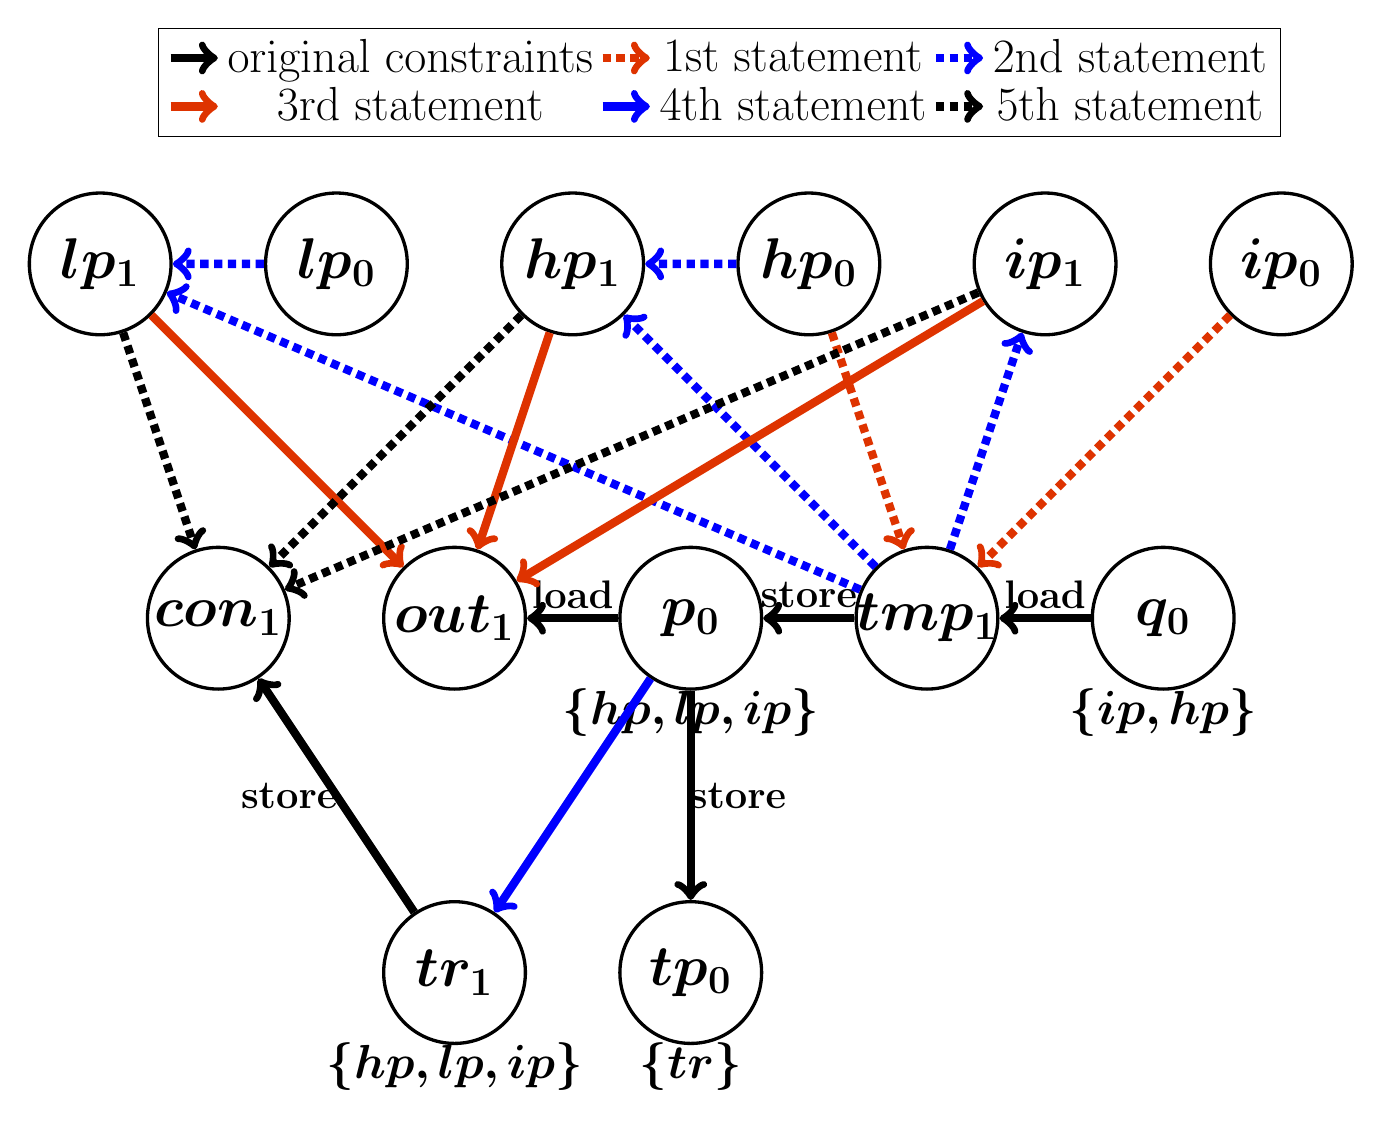
\begin{tikzpicture}[scale=3]
	\tikzstyle{every node}=[circle,draw,minimum size=1.8cm,very thick]
	\node (con1) at (0,0) {};
	\node (out) at (1,0) {};
	\node (p) at (2,0) {};
	\node (t) at (3,0) {};
	\node (q) at (4,0) {};
	\node (tp) at (2,-1.5) {};
	\node (tr1) at (1,-1.5) {};
	\node (hp1) at (1.5,1.5) {};
	\node (hp0) at (2.5,1.5) {};
	\node (lp1) at (-0.5,1.5) {};
	\node (lp0) at (0.5,1.5) {};
	\node (ip1) at (3.5,1.5) {};
	\node (ip0) at (4.5,1.5) {};
    \tikzstyle{every node}=[draw=none,font=\huge]
	\node () at (2,0) {$\bm{p_0}$};
	\node () at (0,0) {$\bm{con_1}$};
	\node () at (1,0) {$\bm{out_1}$};
	\node () at (3,0) {$\bm{tmp_1}$};
	\node () at (4,0) {$\bm{q_0}$};
	\node () at (2,-1.5) {$\bm{tp_0}$};
	\node () at (1,-1.5) {$\bm{tr_1}$};
	\node () at (1.5,1.5) {$\bm{hp_1}$};
	\node () at (2.5,1.5) {$\bm{hp_0}$};
	\node () at (-0.5,1.5) {$\bm{lp_1}$};
	\node () at (0.5,1.5) {$\bm{lp_0}$};
	\node () at (3.5,1.5) {$\bm{ip_1}$};
	\node () at (4.5,1.5) {$\bm{ip_0}$};
    \tikzstyle{every node}=[draw=none,font=\LARGE]
    \node () at (4,-0.4) {$\bm{\{ip,hp\}}$};
    \node () at (2,-0.4) {$\bm{\{hp,lp,ip\}}$};
    \node () at (2,-1.9) {$\bm{\{tr\}}$};
    \node () at (1,-1.9) {$\bm{\{hp,lp,ip\}}$};
	\draw[->,line width=3pt] (q) -- (t) node[draw=none,font=\Large] at (3.5,0.1) {\textbf{load}};
	\draw[->,line width=3pt] (t) -- (p) node[draw=none,font=\Large] at (2.5,0.1) {\textbf{store}};
	\draw[->,line width=3pt] (p) -- (out) node[draw=none,font=\Large] at (1.5,0.1) {\textbf{load}};
	\draw[->,line width=3pt] (p) -- (tp) node[draw=none,font=\Large] at (2.2,-0.75) {\textbf{store}};
	\draw[->,line width=3pt] (tr1) -- (con1) node[draw=none,font=\Large] at (0.3,-0.75) {\textbf{store}};
	\draw[dotted,red,->,line width=3pt] (ip0) -- (t);
	\draw[dotted,red,->,line width=3pt] (hp0) -- (t);
	\draw[dotted,blue,->,line width=3pt] (hp0) -- (hp1);
	\draw[dotted,blue,->,line width=3pt] (lp0) -- (lp1);
	\draw[dotted,blue,->,line width=3pt] (t) -- (hp1);
	\draw[dotted,blue,->,line width=3pt] (t) -- (lp1);
	\draw[dotted,blue,->,line width=3pt] (t) -- (ip1);
	\draw[red,->,line width=3pt] (hp1) -- (out);
	\draw[red,->,line width=3pt] (lp1) -- (out);
	\draw[red,->,line width=3pt] (ip1) -- (out);
	\draw[blue,->,line width=3pt] (p) -- (tr1);
	\draw[dotted,->,line width=3pt] (hp1) -- (con1);
	\draw[dotted,->,line width=3pt] (lp1) -- (con1);
	\draw[dotted,->,line width=3pt] (ip1) -- (con1);
\begin{customlegend}[
legend entries={ % <= in the following there are the entries
original constraints,
1st statement,
2nd statement,
3rd statement, 
4th statement,
5th statement,
},
legend columns=3,
legend style={at={(4.5,2.5)},font=\footnotesize}] % <= to define position and font legend
% the following are the "images" and numbers in the legend
    \addlegendimage{->,line width=3pt}
    \addlegendimage{dotted,red,->,line width=3pt}
    \addlegendimage{dotted,blue,->,line width=3pt}
    \addlegendimage{red,->,line width=3pt}
    \addlegendimage{blue,->,line width=3pt}
    \addlegendimage{dotted,->,line width=3pt}
\end{customlegend}
	\end{tikzpicture}
    }
    \begin{center}
    (d) Final constraint graph after FSCS analysis
    \end{center}
    &
\hspace{1.1cm}
    \scalebox{0.4}{
	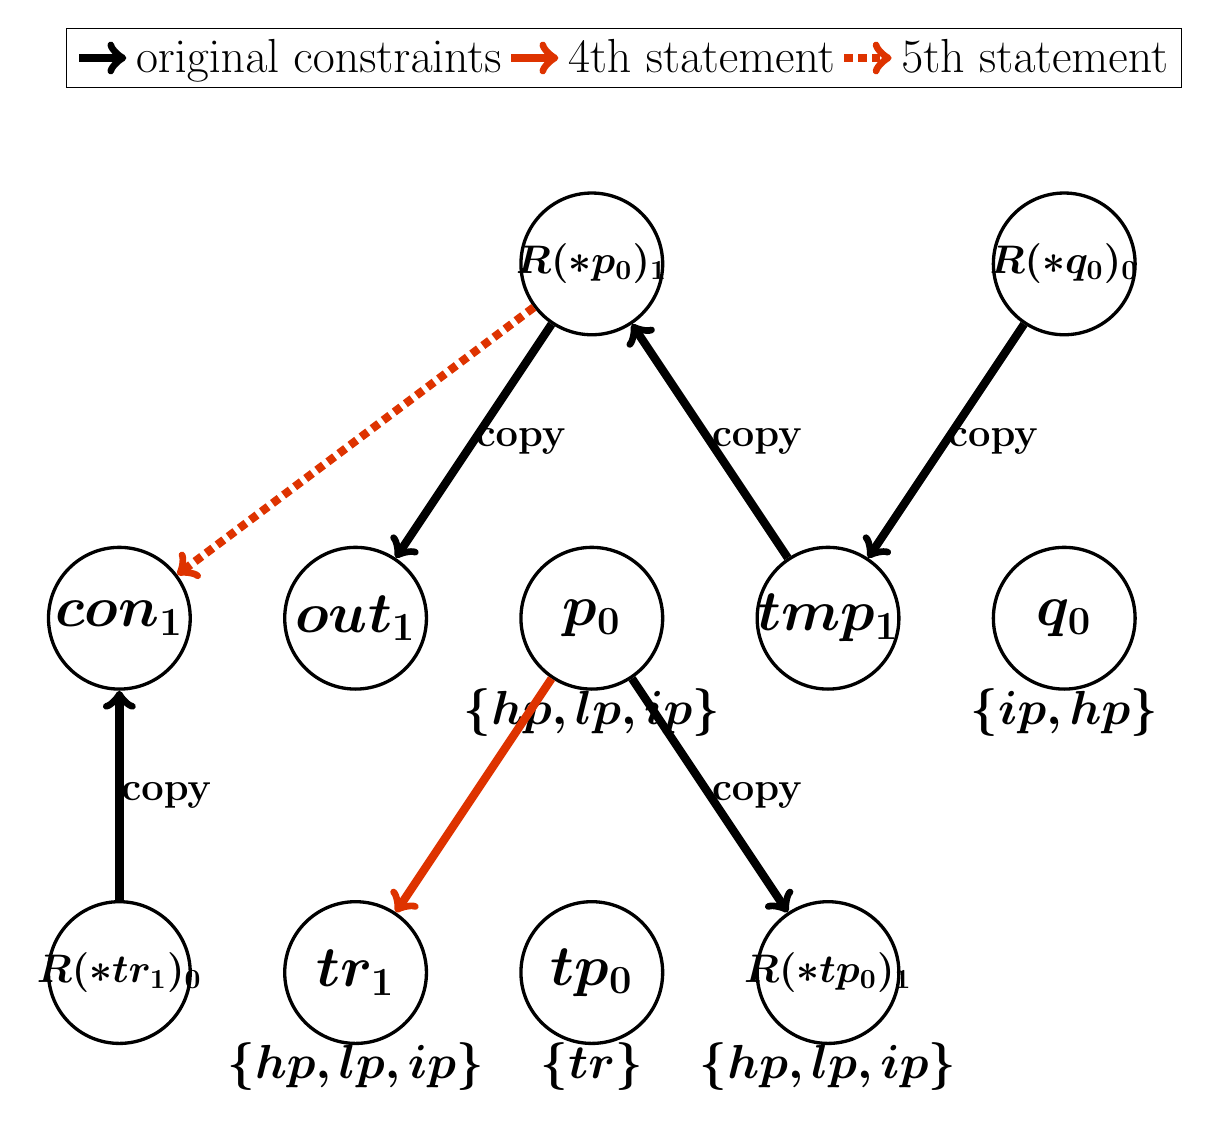
\begin{tikzpicture}[scale=3]
	\tikzstyle{every node}=[circle,draw,minimum size=1.8cm,very thick,font=\huge]
	\node (con1) at (0,0) {};
	\node (out) at (1,0) {};
	\node (p) at (2,0) {};
	\node (t) at (3,0) {};
	\node (q) at (4,0) {};
	\node (tp) at (2,-1.5) {};
	\node (*tp01) at (3,-1.5) {};
	\node (tr1) at (1,-1.5){};
	\node (*tr10) at (0,-1.5) {};
	\node (*p01) at (2,1.5) {};
	\node (*q00) at (4,1.5) {};
    \tikzstyle{every node}=[draw=none,font=\huge]
	\node () at (0,0) {$\bm{con_1}$};
	\node () at (1,0) {$\bm{out_1}$};
	\node () at (2,0) {$\bm{p_0}$};
	\node () at (3,0) {$\bm{tmp_1}$};
	\node () at (4,0) {$\bm{q_0}$};
	\node () at (2,-1.5) {$\bm{tp_0}$};
	\node () at (1,-1.5){$\bm{tr_1}$}{};
    \tikzstyle{every node}=[draw=none,font=\Large]
	\node () at (3,-1.5) {$\bm{R(*tp_0)_1}$};
	\node () at (0,-1.5) {$\bm{R(*tr_1)_0}$};
	\node () at (2,1.5) {$\bm{R(*p_0)_1}$};
	\node () at (4,1.5) {$\bm{R(*q_0)_0}$};
    \tikzstyle{every node}=[draw=none,font=\LARGE]
    \node () at (4,-0.4) {$\bm{\{ip,hp\}}$};
    \node () at (2,-0.4) {$\bm{\{hp,lp,ip\}}$};
    \node () at (2,-1.9) {$\bm{\{tr\}}$};
    \node () at (1,-1.9) {$\bm{\{hp,lp,ip\}}$};
    \node () at (3,-1.9) {$\bm{\{hp,lp,ip\}}$};
    \draw[->,line width=3pt] (p) -- (*tp01) node[draw=none,font=\Large] at (2.7,-0.75) {\textbf{copy}};
	\draw[->,line width=3pt] (*q00) -- (t) node[draw=none,font=\Large] at (3.7,0.75) {\textbf{copy}};
	\draw[->,line width=3pt] (t) -- (*p01) node[draw=none,font=\Large] at (2.7,0.75) {\textbf{copy}};
	\draw[->,line width=3pt] (*p01) -- (out) node[draw=none,font=\Large] at (1.7,0.75) {\textbf{copy}};
	\draw[->,line width=3pt] (*tr10) -- (con1) node[draw=none,font=\Large] at (0.2,-0.75) {\textbf{copy}};
	\draw[red,->,line width=3pt] (p) -- (tr1);
	\draw[dotted,red,->,line width=3pt] (*p01) -- (con1);
\begin{customlegend}[
legend entries={ % <= in the following there are the entries
original constraints,
4th statement,
5th statement,
},
legend columns=3,
legend style={at={(4.5,2.5)},font=\footnotesize}] % <= to define position and font legend
% the following are the "images" and numbers in the legend
    \addlegendimage{->,line width=3pt}
    \addlegendimage{red,->,line width=3pt}
    \addlegendimage{dotted,red,->,line width=3pt}
\end{customlegend}
	\end{tikzpicture}
    }
    \begin{center}
    (e) Final constraint graph after our strong updates analysis
    \end{center}
    \\
\hline \hline
%Points-to map results
\hspace{5em}    \begin{tabular}{l}
\\
    $\ptrset{(tmp_1)} = \{high,in)\}$\\
	$\ptrset{(hp_1)} = \{high,in\}$\\
    $\ptrset{(lp_1)} = \{in,low\}$\\
    $\ptrset{(ip_1)} = \{high,in\}$\\
	$\ptrset{(out_1)} = \{high,in,low\}$\\
    $\ptrset{(tr_1)} = \{high,in,low\}$\\
	$\ptrset{(con_1)} = \{high,in,low\}$\\
    \end{tabular}
    &
\hspace{5em}    \begin{tabular}{l}
\\
    $\ptrset{(tmp_1)} = \{high,in\}$\\
    $\ptrset{(R(*p_0)_1)} = \{high,in\}$\\
    $\ptrset{(R(*tr_1)_1)} = \{high,in\}$\\
	$\ptrset{(out_1)} = \{high,in\}$\\
	$\ptrset{(R(*tp_0)_1)} = \{high,in,low\}$\\
    $\ptrset{(tr_1)} = \{high,in,low\}$\\
    $\ptrset{(con_1)} = \{high,in\}$\\
    \end{tabular}
\\
    \begin{center}
    (f) Points-to set of SSA variables after FSCS analysis
    \end{center}
    &
    \begin{center}
    (g) Points-to set of regions after our strong updates analysis
    \end{center}\\
\hline
\end{tabular}
\end{center}
\caption{TO BE DEFINED}
\label{fig:comparison}
\end{figure*}




	
\begin{figure*}
\centering
\hspace*{-8mm}
\begin{tabular}{l@{\hspace{8mm}}l@{\hspace{8mm}}l}


Analyzing-Level: & $e' \parorder e$ \hspace{2mm} $e' \parordereq e$  \hspace{2mm} $ \curana{e} $
&
\begin{tabular}{l} $e' \parorder e$: expression $e'$ is analyzed before $e$ \\
$e' \parordereq e$: expression $e'$ is analyzed togeter with $e$ \\
$ \curana{e} $ stands for current under analyzing expr, \\
higher level exprs are solved and SSA-renamed.
\end{tabular}.
\\\\


Points-to Map: & $(v,C,M) \in \ptr(R)$
&
\begin{tabular}{l} Region $R$ points to $v$ at context condition $C$ \\ the points-to must hold under condition $M$ \end{tabular}.

\\\\

Region Aliases: & $(v,C,M) \in \alias(R)$
&
\begin{tabular}{l} Memory locaion $v$ is represented by $R$ \\ under context condition $C$ and condition $M$  \end{tabular}.

\\\\


Sparse-Resolution: & $\vdash \stmt{s}^\re_\mo \ptsinf \pts{\underline{s}}$
&
\begin{tabular}{l}Given annotated $\mu$ and $\chi$ at stmt $s$ \\to produce sparse points-to relations after $s$ \end{tabular}.

\\\\

Points-to Relations: & $\pts{\underline{s}}(p_i) \equiv \ptr(p_i) \equiv \alias(*p_i)$
&
\begin{tabular}{l}  Points-to relations \end{tabular}.

\\\\

Points-to Set: & $v \in \ptrset{(p_i)}$
&
\begin{tabular}{l} Points-to set  \end{tabular}.

\\\\

Mod-Ref: & $\vdash f \modrefinf \refset; \modset $  \ruleindent $\vdash s \modrefinf \refset; \modset $
&
\begin{tabular}{l} $\modset/\refset$ is mod/ref regions that contain variables \\ maybe indirectly modified/read in $f$ or at $s$,\end{tabular}.

\\\\


Proc-Trans-Effect: & $\vdash f \transinf \modset \tfinf \trans{f}$
&
\begin{tabular}{l} Build transfer function $\trans{f}$ for \\ mod regions $\modset$ in procedure $f$ \end{tabular}.
 \\\\


Proc-Meet-Effect: & $\vdash f \transinf \refset \tfinf \meet{f}$
&
\begin{tabular}{l} Build meet function $\meet{f}$ for \\ ref regions $\refset$ in procedure $f$ \end{tabular}.
 \\\\

Eval-Call-Mod: & $\vdash R_i \evaltfinf \textsf{call}_k : \ptr(R_i)$
&
\begin{tabular}{l} Evaluate points-to for \\ mod region $R_i$ at callsite $\textsf{call}_k$\end{tabular}.
 \\\\


CS-Callee-Map: & $\vect{f} = \Mapcs(\textsf{call}_{k})$ \hspace{3mm} $\vect{\textsf{call}_{k}} = \Mapproc(f)$
&
\begin{tabular}{l} Map callsite $\textsf{call}_{k}$ to a list of callees $\vect{f}$.\\
Map $f$ to a list of invocation callsites $\vect{\textsf{call}_{k}}$
\end{tabular}
\\\\

Region-Map: & $R \underset{call_k}{\overset{f}{\looparrowright}} R'$
&
\begin{tabular}{l} Map region R through callsite \textsf{call$_k$} \\ to region R' in callee $f$ when TF Evaluation \end{tabular}.
\\\\

Condition-Map: & $C \underset{call_k}{\overset{f}{\leadsto}} \Ddot{C}$ \hspace{3mm} $M \underset{call_k}{\overset{f}{\leadsto}} \Ddot{M}$
&
\begin{tabular}{l} Map condition $C/M$ from callee $f$ to \\ callsite \textsf{call$_k$}  when TF Evaluation \end{tabular}.
\\\\




\end{tabular}
\caption{Semantics Definitions.
\label{fig:lang}}
\end{figure*}

\begin{figure*}[h]
\centering
\setlength{\tabcolsep}{1.1ex}
%\def\arraystretch{1.16}
%\rulefont
\begin{tabular}{l}

\begin{tabular}{l@{\hspace{0.2mm}}l}
\ruledef{\rulefont I-PROC}{
\begin{tabular}{llll}
$\vdash$ \emph{f} \modrefinf $\refset; \modset$

\ruleindent $\vect{s} = \Unfoldproc(f)$
\ruleindent $\vdash \vect{s} \modrefinf \vect{\CSU}; \vect{\CSD}$
\\

\end{tabular}
}{
\begin{tabular}{l}
$\refset=\bigcup_{\vect{\refset}}$ \ruleindent $\modset = \bigcup_{\vect{\CSD}}$
\end{tabular}
}
\end{tabular}

\\\\

\begin{tabular}{l@{\hspace{-0.3mm}}l}
\ruledef{\rulefont I-CALL}{
\begin{tabular}{lll}
$\vdash$ \textsf{call}$_{k}$ \modrefinf $\CSU; \CSD$
\ruleindent $\vect{f} = \Mapcs$(\textsf{call$_{k}$})
\ruleindent $\vdash \vect{f} \modrefinf \vect{\refset};\vect{\modset}$\\

\end{tabular}
}{
\begin{tabular}{l}
$\refset = (\bigcup_{\vect{\refset}}) \cap \PTG_{{\sf call}_k}$  $\modset = (\bigcup_{\vect{\modset}}) \cap \PTG_{\textsf{call}_k}$
\end{tabular}
}
\end{tabular}




\\\\

\begin{tabular}{l@{\hspace{-0.5mm}}l@{\hspace{-0.5mm}}ll}

\ruledef{\rulefont i-ld}{
\label{rule:ld}
\begin{tabular}{lll}
$\vdash p=*q_i \modrefinf \refset; \modset $
\ruleindent $R(*q_i) = \ptrset{(q_i)}$
\ruleindent $\curana{q} \parorder *q \parordereq p$\\
\ruleindent $v \in R(*q_i)$ \hspace{1mm} $v$ is nonlocal
\end{tabular}
}{
\begin{tabular}{l}
$\refset = \{R(*q_i)\}$ \ruleindent $\modset = \emptyset$
\end{tabular}
}

\\\\

\ruledef{\rulefont i-st}{
\label{rule:st}
\begin{tabular}{lll}
$\vdash *p_i=q \modrefinf \refset; \modset $
\ruleindent $R(*p_i) = \ptrset{(p_i)}$
\ruleindent $\curana{p} \parorder *p \parordereq q$\\
\ruleindent $v \in R(*p_i)$ \hspace{1mm} $v$ is nonlocal
\end{tabular}
}{
\begin{tabular}{l}
$\refset = \emptyset$ \ruleindent  $\modset = \{R(*p_i)\}$
\end{tabular}
}
\end{tabular}

\\\\

\begin{tabular}{l@{\hspace{-0.5mm}}l@{\hspace{-0.5mm}}ll}
\ruledef{\rulefont i-add}{
\label{rule:ad}
\begin{tabular}{lll}
$\vdash p=\&q \modrefinf \refset; \modset $  \ruleindent $p \parordereq \&q \parorder q$
\end{tabular}
}{
\begin{tabular}{ll}
$\refset = \emptyset$ \ruleindent $\modset = \emptyset$
\end{tabular}
}

\hspace{-3mm}
\ruledef{\rulefont i-asn}{
\label{rule:as}
\begin{tabular}{lll}
$\vdash p=q \modrefinf \refset; \modset  $  \ruleindent $p \parordereq q$
\end{tabular}
}{
\begin{tabular}{ll}
$\refset = \emptyset$ \ruleindent  $\modset = \emptyset $

\end{tabular}
}

\end{tabular}

\\\\


\begin{tabular}{ll}
\ruledef{I-RET}{
	\begin{tabular}{@{\hspace*{-1ex}}lll}
		$\vdash \textsf{return}_{j}(v) \modrefinf \refset; \modset$  \\
\end{tabular}
}{
\begin{tabular}{ll}
$\refset = \emptyset$ \ruleindent $\modset = \{v\}$
\end{tabular}
}
\end{tabular}

\end{tabular}

\caption{Rules used for Mod-Ref analysis and allocating regions for level $lev + 1$ with renamed $lev$ expressions.
\label{fig:rules_mod-ref}}
\end{figure*}





\begin{figure*}[h]

\centering

\begin{tabular}{l@{\hspace{-0.5mm}}l}


\begin{tabular}{l@{\hspace{-0.2mm}}l@{\hspace{-0.2mm}}ll}
\ruledef{M-ADD}{
\begin{tabular}{lll}
$\stmt{p=\&q}^\re_\mo$  	\ruleindent $p \parordereq \&q \parorder q$\\
\end{tabular}
}{
\begin{tabular}{ll}
$\re = \mo = \emptyset$

\end{tabular}
}


\ruledef{M-ASN}{
\begin{tabular}{lll}
$\stmt{p=q}^\re_\mo$ \ruleindent $p \parordereq q$
\end{tabular}
}{
\begin{tabular}{ll}

$\re = \mo = \emptyset$

\end{tabular}
}

\end{tabular}

\\\\

\begin{tabular}{l@{\hspace{-0.2mm}}l}
\ruledef{M-LD}{
\begin{tabular}{lll}
$\stmt{p=R(*q_i)}^\re_\mo$ \ruleindent
$\reg \in \Regs$ \ruleindent $\reg \cap R(*q_i) \ne \emptyset$
\ruleindent $\curana{q} \parorder *q \parordereq p$\\
$(v,C_i,M_i) \in \alias(R)$ \ruleindent$(v,C_j,M_j) \in \alias(R(*q_i))$\\
\end{tabular}
}{
\begin{tabular}{ll}
$\re \cupunion \{\mu(\reg, C_i\wedge C_j, M_i \wedge M_j)\}$ \ruleindent $\mo = \emptyset$

\end{tabular}
}
\end{tabular}

\\
\\

\begin{tabular}{l@{\hspace{-0.2mm}}l}
\ruledef{M-ST}{
\begin{tabular}{lll}
	$\stmt{R(*p_i)=q}^\re_\mo$ \ruleindent $R \in \Regs$ \ruleindent $\reg \cap R(*p_i) \ne \emptyset$
\ruleindent $\curana{p} \parorder *p \parordereq p$\\
	
	$(v,C_i,M_i) \in \alias(R)$ \ruleindent $(v,C_j,M_j) \in \alias(R(*p_i))$\\
	
\end{tabular}
}{
\begin{tabular}{ll}

$\re = \emptyset$ \ruleindent $\mo \cupunion \{\reg = \chi(R, C_i\wedge C_j, M_i \wedge M_j)\}$
\end{tabular}
}
\end{tabular}

\\
\\

\begin{tabular}{l@{\hspace{-0.2mm}}l}
\ruledef{M-CALL}{
\begin{tabular}{lll}
$\stmt{\textsf{call}_{k}}^\re_\mo$
\ruleindent $\vdash \textsf{call}_{k} \modrefinf \refset; \modset$
\ruleindent $\vdash \textsf{call}_{k} \evaltfinf \refset; \meet{\textsf{call}_{k}} $
\ruleindent $\vdash \textsf{call}_{k} \evaltfinf \modset; \trans{\textsf{call}_{k}} $
\\

 $\reg \in \refset$  \ruleindent $\ptr(\reg) \in \meet{\textsf{call}_{k}}$ \ruleindent $(v_i,C_i,M_i) \in \ptr(R)$  \\

$\reg' \in \modset$  \ruleindent $\ptr(\reg') \in \trans{\textsf{call}_{k}}$ \ruleindent $(v_j,C_j,M_j) \in \ptr(R')$\\

\end{tabular}
}{
\begin{tabular}{ll}
$\re \cupunion \{\mu(\reg,C_i,M_i)\}$ \ruleindent  $\mo \cupunion \{\reg' = \chi(\reg',C_j,M_j)\}$
\end{tabular}
}
\end{tabular}

\\
\\


\end{tabular}
\caption{Rules used for annotating the
	indirect defs and uses at a statement
	with $\mu$ and $\chi$ functions when building full-sparse SSA (top-down analysis).
\label{fig:rules_old_ssa}}

\end{figure*}







\begin{figure*}[t]
\centering
%\rulefont
\begin{tabular}{l@{\hspace{1.5mm}}l}




\begin{tabular}{l@{\hspace{0.2mm}}l@{\hspace{0.2mm}}ll}
\ruledef{S-ADD}{
\begin{tabular}{lll}
$\vdash \stmt{p_i \stackleftarrow{\fs s} \&q}^\emptyset_\emptyset \ptsinf \pts{\underline{s}}$
\ruleindent  	$\curana{p} \parordereq \&q \parorder q$
\end{tabular}
}{
\begin{tabular}{ll}
$\pts{\underline{s}}(p_i) = \{(q,\true,\true)\}$

\end{tabular}
}


\ruledef{S-ASN}{
\begin{tabular}{lll}
$\vdash \stmt{p_i \stackleftarrow{\fs s} q_j}^\emptyset_\emptyset \ptsinf \pts{\underline{s}}$
\ruleindent  	$\curana{p} \parordereq \curana{q}$
\end{tabular}
}{
\begin{tabular}{ll}

$\pts{\underline{s}}(p_i) = \pts{\overline{s}}(q_j)$

\end{tabular}
}

\end{tabular}

\\\\



\begin{tabular}{ll}
\ruledef{S-PHI}{
\begin{tabular}{l@{\hspace{5mm}}ll}
$\vdash \stmt{R_i \stackleftarrow{\fs s} \Phi(R_j,R_k)}^\emptyset_\emptyset \ptsinf \pts{\underline{s}}$
\ruleindent $(v_j,C_j,M_j) \in \ptr(R_j)$ \ruleindent $(v_k,C_k,M_k) \in \ptr(R_k)$
\\
\end{tabular}
}{
\begin{tabular}{l@{\hspace{2mm}}l}
$\pts{\underline{s}}(R_i) \cupunion \{(v_j,C_j,false)\}$ \ruleindent $\pts{\underline{s}}(R_i) \cupunion \{(v_k,C_k,false)\}$  \\

\end{tabular}
}
\end{tabular}

\\
\\


\begin{tabular}{ll}
\ruledef{S-LD}{
\begin{tabular}{l@{\hspace{5mm}}ll}
$\vdash \stmt{p_i \stackleftarrow{\fs s} R(*q_k)_j}^\re_\emptyset \ptsinf \pts{\underline{s}}$
\ruleindent  	$q \parorder \curana{*q} \parordereq \curana{p}$
\\

\end{tabular}
}{
\begin{tabular}{l@{\hspace{2mm}}l}
$\pts{\underline{s}}(p_i) = \pts{\overline{s}}(R(*q_k)_j) $  \\

\end{tabular}
}
\end{tabular}

\\
\\



\begin{tabular}{ll}
\ruledef{S-ST-W}{
\begin{tabular}{l@{\hspace{5mm}}l@{\hspace{5mm}}l}
	$\vdash \stmt{R(*p_k)_i \stackleftarrow{\fs s} q_j}^\emptyset_\mo \ptsinf \pts{\underline{s}}$ \ruleindent $(v_j,C_j,M_j) \in \ptr(q_j)$
	\ruleindent  	$p \parorder \curana{*p} \parordereq \curana{q}$ \\
	\ruleindent $(R_t=\chi(R_s,C_s,M_s)) \in \mo$ \ruleindent $M \not\eq \true$ \\
\end{tabular}
}{
\begin{tabular}{l@{\hspace{2mm}}l@{\hspace{2mm}}l}

$\pts{\underline{s}}(R(*p_k)_i) = \pts{\overline{s}}(q_j)$
\ruleindent $\pts{\underline{s}}(R_t) \cupunion \pts{\overline{s}}(R_s)$ \\
\ruleindent \ruleindent $\pts{\underline{s}}(R_t) \cupunion \{(v_j, C_j \wedge C_s, M_j \wedge M_s)\}$

\\\end{tabular}
}
\end{tabular}

\\
\\

\begin{tabular}{ll}
\ruledef{S-ST-S}{
\begin{tabular}{l@{\hspace{5mm}}l@{\hspace{5mm}}l}
	$\vdash \stmt{R(*p_k)_i \stackleftarrow{\fs s} q_j}^\emptyset_\mo \ptsinf \pts{\underline{s}}$ \ruleindent $(v_j,C_j,M_j) \in \ptr(q_j)$
		\ruleindent  	$p \parorder \curana{*p} \parordereq \curana{q}$ \\
	\ruleindent $(R_t=\chi(R_s,C_s,M_s)) \in \mo$ \ruleindent $M = \true$ \\
\end{tabular}
}{
\begin{tabular}{l@{\hspace{2mm}}l@{\hspace{2mm}}l}

$\pts{\underline{s}}(R(*p)_i) = \pts{\overline{s}}(q_j)$ \ruleindent $\pts{\underline{s}}(R_t) = \pts{\overline{s}}(q_j)$  \\

\end{tabular}
}
\end{tabular}

\\
\\



\begin{tabular}{ll}
\ruledef{S-CALL-W}{
\begin{tabular}{l@{\hspace{2mm}}l@{\hspace{2mm}}l@{\hspace{2mm}}l}
$\vdash \stmt{\textsf{call}_{k}}^\re_\mo \ptsinf \pts{\underline{\textsf{call}_{k}}}$
\ruleindent $(R_t=\chi(R_s,C_i,M)) \in \mo$  \ruleindent $M \not\eq \true$\\
\ruleindent $\vdash R_t \evaltfinf \textsf{call}_k : \ptr(R_t)$
\ruleindent $(v_t,C_t,M_t) \in \ptr(R_t)$
\\
\end{tabular}
}{
\begin{tabular}{ll}
$\pts{\underline{\textsf{call}_{k}}}(R_t) \cupunion \{(v_t, C_i \wedge C_t, M_i \wedge M_t,)\} $ \ruleindent
$\pts{\underline{\textsf{call}_{k}}}(R_t) \cupunion \pts{\overline{\textsf{call}_{k}}}(R_s) $
\end{tabular}
}
\end{tabular}

\\
\\



\begin{tabular}{ll}
\ruledef{S-CALL-S}{
\begin{tabular}{l@{\hspace{2mm}}l@{\hspace{2mm}}l@{\hspace{2mm}}l}
$\vdash \stmt{\textsf{call}_{k}}^\re_\mo \ptsinf \pts{\underline{\textsf{call}_{k}}}$
\ruleindent  $M=\true$\\
$(R_t=\chi(R_s,C_i,M)) \in \mo$
\ruleindent $\vdash R_t \evaltfinf \textsf{call}_k : \ptr(R_t)$
\\
\end{tabular}
}{
\begin{tabular}{ll}
$\pts{\underline{\textsf{call}_{k}}}(R_t) = \ptr(R_t)$
\end{tabular}
}
\end{tabular}

\\
\\

\end{tabular}
\caption{Rules for pointer resolution.
\label{fig:rules_old_ssa}}

\end{figure*}













\begin{figure*}[t]
\setlength{\tabcolsep}{1.1ex}
%\def\arraystretch{1.16}
\centering
%\rulefont
\begin{tabular}{l@{\hspace{1.5mm}}l}


\begin{tabular}{l@{\hspace{-0.2mm}}l}
\ruledef{S-BUILD-MF}{
\begin{tabular}{lll}
$\vdash f \transinf \refset \tfinf \meet{f}$
\ruleindent $\vect{\textsf{call}_k} = \Mapproc(f)$
\ruleindent $\vdash \vect{\textsf{call}_{k}} \modrefinf \vect{\refset}; \vect{\modset}$
\ruleindent $\vdash \stmt{\vect{\textsf{call}_k}}^\re_\mo \ptsinf \pts{\vect{\overline{\textsf{call}_k}}}$\\
 $\ptr(R_i) \in \pts{\vect{\overline{\textsf{call}_k}}}$ \ruleindent $R_i \cap \vect{\refset} \not\eq\emptyset$\ruleindent $i = min_{ver}$

\end{tabular}
}{
\begin{tabular}{ll}
$!!!\textcolor{red}{M_1} \wedge \textcolor{red}{M_2}, !!!\textcolor{red}{C_1} \vee \textcolor{red}{C_2} \meet{f} \cupunion \ptr(R_i)$\\
\end{tabular}
}
\end{tabular}

\\
\\



\begin{tabular}{ll}
\ruledef{S-BUILD-TF-PROC}{
\begin{tabular}{l@{\hspace{2mm}}l@{\hspace{2mm}}l@{\hspace{2mm}}l}
$\vdash f \transinf \modset \tfinf \trans{f}$ \ruleindent $\vect{s} = \Unfoldproc(f)$ \ruleindent $\vdash \stmt{\vect{s}}^\re_\mo \ptsinf \pts{\underline{s}}$ \\
 $\ptr(R_i) \in \pts{\underline{s}}$
 \ruleindent $\vdash f \modrefinf \refset; \modset$
 \ruleindent $R_i \cap \modset \not\eq\emptyset$\ruleindent $i = max_{ver}$
\end{tabular}
}{
\begin{tabular}{l@{\hspace{2mm}}l}
$\trans{f} \cupunion \ptr(R_i)$\\

\end{tabular}
}

\end{tabular}

\\\\



\begin{tabular}{ll}
\ruledef{S-EVAL-CS}{
\begin{tabular}{l@{\hspace{2mm}}l@{\hspace{2mm}}l@{\hspace{2mm}}l}
\ruleindent $\vdash R_t \evaltfinf \textsf{call}_k : \ptr(R_t)$
\ruleindent $\vect{f} = \Mapcs(\textsf{call}_k)$
\ruleindent $f \in \vect{f}$
\\
%$\vdash R \evaltfinf \trans{f} \applytfinf \ptr(R)$
\ruleindent $\vdash f \transinf \modset' \tfinf \trans{f}$
\ruleindent $R' \in \modset'$
\ruleindent $R_t\looparrowright_f^{call_k} R'$
\ruleindent  $\ptr(R') \in \trans{f}$\\
\ruleindent $(v_i,C_i,M_i) \in \ptr(R')$
\ruleindent $C_i \leadsto_f^{call_k} \Ddot{C_i}$
\ruleindent $M_i \leadsto_f^{call_k} \Ddot{M_i}$
\ruleindent $\Ddot{C_i}$ holds at $\textsf{call}_{k}$
\end{tabular}
}{
\begin{tabular}{ll}
$\ptr(R_t) \cupunion \{(v_i,\Ddot{C_i},\Ddot{M_i})\}$
\end{tabular}
}
\end{tabular}

\\
\\


%
%\begin{tabular}{ll}
%\ruledef{S-RET}{
%	\begin{tabular}{@{\hspace*{-1ex}}lll}
%		$\stmt{\textsf{return}_{j}}^\re_\emptyset$   $\hspace{1mm}$ $\vdash \emph{f} : \CSU,\CSD$\hspace*{0ex}
%		$\reg \in \Regs_f$  \hspace*{0ex}$ \reg \cap \CSD \ne \emptyset$ \\
%\end{tabular}
%}{
%\begin{tabular}{ll}
%$\re \cupunion \{\mu(\reg)$\}  & $\mo = \emptyset$
%\end{tabular}
%}
%\end{tabular}



\end{tabular}
\caption{Rules for building meet/transfer functions at callsites (bottom-up analysis).
\label{fig:rules_old_ssa}}

\end{figure*}


\end{comment}




\section{Related Works}

%\cite{zhu2004symbolic} analysis is fully symbolic (everything from the CFG to the pointer information is represented using BDDs) but not fully flow-sensitive�the analysis cannot perform indirect strong updates, so the KILL sets are more conservative (i.e., smaller) than a fully flow-sensitive analysis\cite{hardekopf2009semi,hardekopfflow}. 



%\appendix
%\section{Appendix Title}

%This is the text of the appendix, if you need one.

\bibliography{strongupdates}

\bibliographystyle{plain}

% The bibliography should be embedded for final submission.




\end{document}

%%%%%%%%%%%%%%%%%%%%%%%%%%
%discarded texts
%%%%%%%%%%%%%%%%%%%%%%%%%%
\begin{center}
\begin{table}
	\begin{tabular}{|rcl|l|}
	\hline
	$p$ & = & $\&x$ & $\ptrmap{p} = \{(x, T, T)\}$ \\ \hline
	$p$ & = & $q$ & $\ptrmap{p} = \ptrmap{q}$ \\ \hline
	$p$ & = & $*q$ & $\ptrmap{p} = \ptrmap{R(*q)}$ \\ \hline
	$*p$ & = & $q$ & $\ptrmap{R(*p)} = \ptrmap{q}$ \\ \hline
	$R(*p)_2$ & = & $\chi(R(*p)_1)$ & \\ \hline
	$p_3$ & = & $\phi(p_1, p_2)$ & $\ptrmap{p_3} = \{(x,C,false)|(x,C,M) \in \ptrmap{p_1} \vee (x,C,M) \in \ptrmap{p_2}\}$ \\ \hline
	\end{tabular}
\end{table}
\end{center}

\begin{table}[h]
\begin{center}
	\begin{tabular}{|rcl|l|}
    \hline
		$R(*p)_1$ & = & $R(*q)_0$; & \ptrmap{$R(*p)_1$} = $\{(g,C_1,M),(l,C_2,M)\}$\\
		$R(*q)_1$ & = & malloc(4); & \ptrmap{$R(*q)_1$} = $\{(o,T,M)\}$\\
		$j_1$ & = & $R(*p)_1$; & \ptrmap{$R(j)_1$} = $\{(g,C_1,M),(l,C_2,M)\}$\\
		$R(*r)_1$ & = & $p_0$; & \ptrmap{$R(*r)_1$} = $\{(x,C_1,M),(y,C_1,M),(z,C_2,M)\}$\\
        $\bm{R(s)_1}$ & \textbf{=} & $\bm{\chi(R(s)_0)}$ & \ptrmap{$R(s)_1$} = $\{(x,C_1,M),(y,C_1,M),(z,C_2,M)\}$\\
        $h_1$ & = & $R(*s)_1$; & \ptrmap{$R(h)_1$} = $\{(g,C_1,M),(l,C_2,M)\}$\\
    \hline \hline
		*p & = & *q; & \ptrmap{x} = $\{(m,C_1,M),(g,C_1,M)\}$\\
        & & & \ptrmap{y} = $\{(n,C_1,M),(g,C_1,M)\}$\\
        & & & \ptrmap{z} = $\{(l,C_2,M)\}$\\
		*q & = & malloc(4); & \ptrmap{h} = $\{(g,C_1,M),(o,C_1,M)\}$\\
        & & & \ptrmap{z} = $\{(l,C_2,M),(o,C_2,M)\}$\\
		j & = & *p; & \ptrmap{j} = $\{(m,C_1,M),(n,C_1,M),(l,C_1,M),(g,C_2,M)\}$\\
		*r & = & p; & \ptrmap{s} = $\{(x,C_1,M),(y,C_1,M),(z,C_2,M)\}$\\
		h & = & *s; & \ptrmap{h} = $\{(m,C_1,M),(n,C_1,M),(l,C_1,M),(g,C_2,M)\}$\\
    \hline
	\end{tabular}
\end{center}
\caption{Differences between traditional flow-sensitive analysis and our memory region based strong update analysis in foo function.}
\label{table:result comparison}
\end{table}

\begin{table}[h]
\begin{center}
	\begin{tabular}{|r|l|}
		\hline
		\multirow{3}{*}{
			\begin{tabular}{r}
				CS1: foo(a, b, c);\\
			\end{tabular}
		}
		&	\begin{tabular}{l}
				\ptrmap{x} = $\{(m,T,M),(g,T,M)\}$\\
				\ptrmap{y} = $\{(n,T,M),(g,T,M)\}$\\
				\ptrmap{j} = $\{(g,T,M)\}$\\
				\ptrmap{h} = $\{(g,T,M)\}$\\
				\ptrmap{s} = $\{(x,T,M),(y,T,M)\}$\\
			\end{tabular} \\ \cline{2-2}
		&	\begin{tabular}{l}
			\end{tabular} \\ \cline{2-2}
		&	\begin{tabular}{l}
			\end{tabular}\\
		\hline \hline
		\multirow{3}{*}{
			\begin{tabular}{r}
				CS2: foo(a, b, c);\\
			\end{tabular}
		}
		&	\begin{tabular}{l}
				\ptrmap{z} = $\{(m,T,M),(g,T,M)\}$\\
			\end{tabular} \\ \cline{2-2}
		&	\begin{tabular}{l}
			\end{tabular} \\ \cline{2-2}
		&	\begin{tabular}{l}
			\end{tabular}\\
		\hline
	\end{tabular}
\end{center}
\caption{Differences between FSCI, FSCS and our memory region based strong update analysis at call sites in main function.}
\end{table}

\begin{figure}
\begin{center}
	\begin{tabular}{p{8cm}p{8cm}}
	\begin{lstlisting}[name=Result,mathescape]
int g, *h, *j, *s;
void main()
{
  int m, n, l;
  int *x, *y, *z;
  int **a, **b, **c;
  $x_1$ = &m, $y_1$ = &n, $z_1$ = &l;
  $h_1$ = &g;
  if (*) $a_1$ = &x;
  else   $a_2$ = &y;
  $a_3$ = $\phi(a_1, a_2)$
  $b_1$ = &h, $c_1$ = &s, $s_1$ = &z;

      $\mu(x_1)$
      $\mu(y_1)$
      $\mu(h_0)$
      $\mu(s_1)$
  foo($a_3$, $b_1$, $c_1$);
  $x_2 = \chi(x_1)$
  $y_2 = \chi(y_1)$
  $h_2 = \chi(h_1)$
  $s_2 = \chi(s_1)$

  $a_4$ = &z, $b_2$ = $a_4$;

      $\mu(z)$
      $\mu(s)$
  foo($a_4$, $b_2$, $c_1$);
  $z_1 = \chi(z_0)$
  $s_3 = \chi(s_2)$
}
	\end{lstlisting}
	&
	\begin{lstlisting}[name=Result,mathescape]
void foo(int **p, int **q, int **r)
{
	  $\mu(h_0)$
	  $\mu(z_0)$
  $t_1 = *q_0$;

  $*p_0$ = $t_1$;
  $x_1 = \chi(x_0)$
  $y_1 = \chi(y_0)$
  $z_1 = \chi(z_0)$

  $*q_0$ = malloc(4);
  $h_1 = \chi(h_0)$
  $z_2 = \chi(z_1)$

	  $\mu(x_1)$
	  $\mu(y_1)$
	  $\mu(z_2)$
  $j_1$ = $*p_0$;

  $*r_0$ = $p_0$;
  $s_1 = \chi(s_0)$

	  $\mu(x_1)$
	  $\mu(y_1)$
	  $\mu(z_2)$
  $h_2$ = $*s_1$;
}
	\end{lstlisting}
	\end{tabular}
\end{center}
\caption{SSA form after traditional flow- and context-sensitive analysis}
\label{fig:SSA form of FSCS analysis}
\end{figure}

\begin{figure}
\begin{center}
\scalebox{0.4}{
	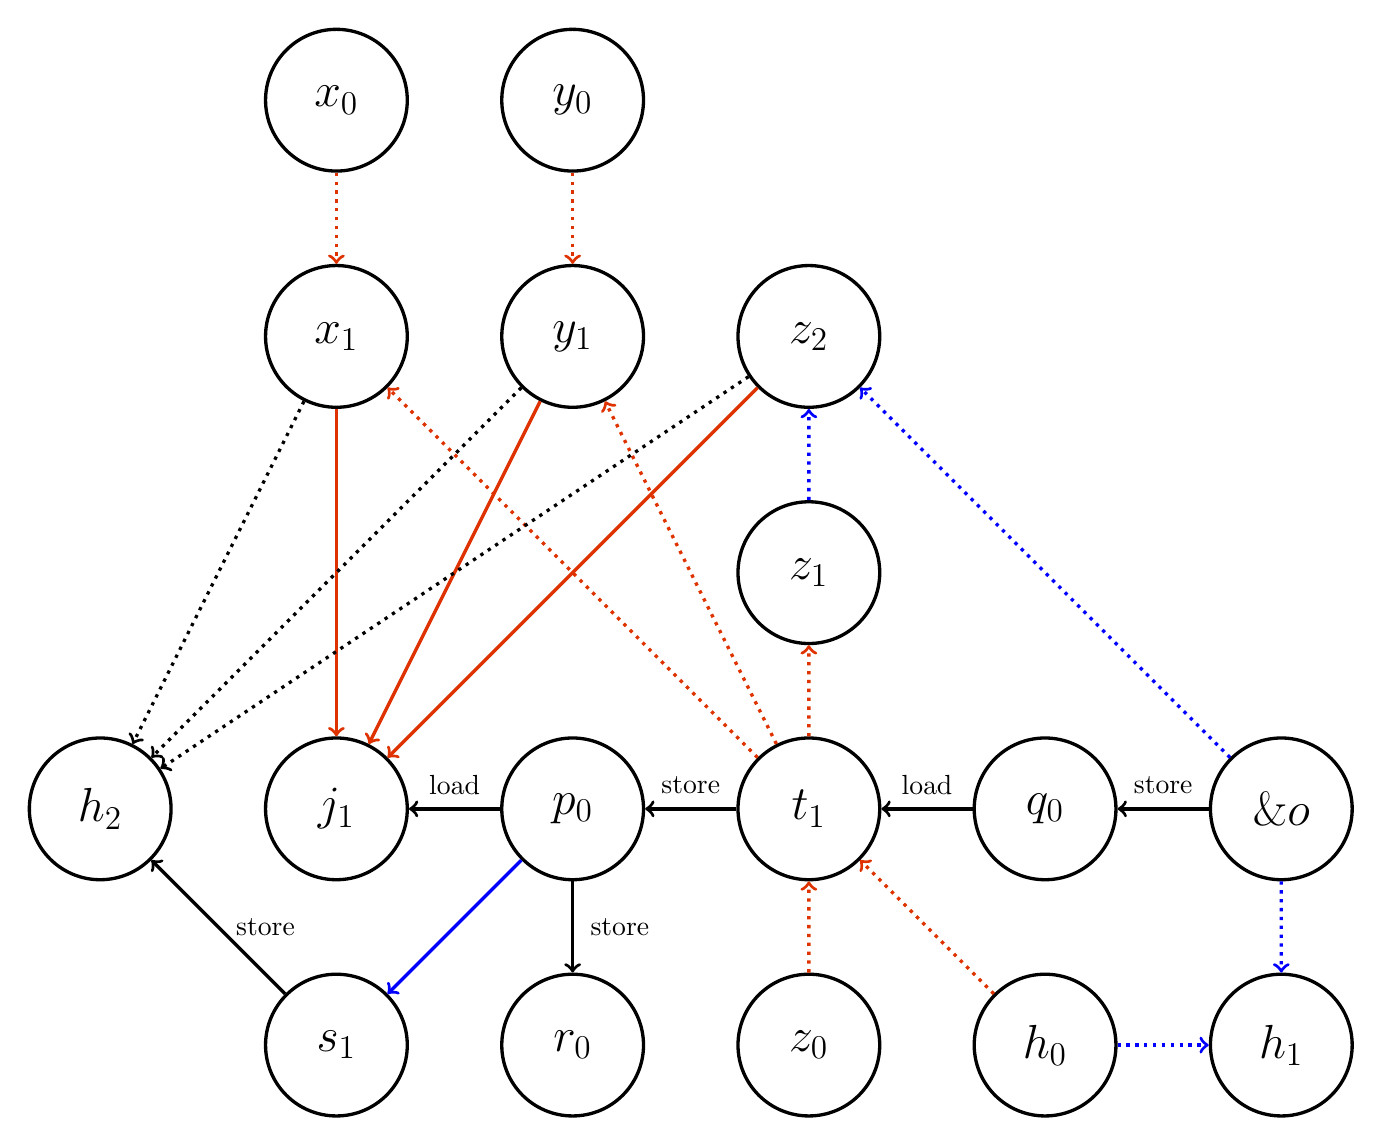
\begin{tikzpicture}[scale=3]
	\tikzstyle{every node}=[circle,draw,minimum size=1.8cm,very thick,font=\LARGE]
	\node (h2) at (-1,0) {$h_2$};
	\node (j) at (0,0) {$j_1$};
	\node (p) at (1,0) {$p_0$};
	\node (t) at (2,0) {$t_1$};
	\node (q) at (3,0) {$q_0$};
	\node (o) at (4,0) {$\&o$};
	\node (r) at (1,-1) {$r_0$};
	\node (s1) at (0,-1) {$s_1$};
	\node (x1) at (0,2) {$x_1$};
	\node (x0) at (0,3) {$x_0$};
	\node (y1) at (1,2) {$y_1$};
	\node (y0) at (1,3) {$y_0$};
	\node (z2) at (2,2) {$z_2$};
	\node (z1) at (2,1) {$z_1$};
	\node (z0) at (2,-1) {$z_0$};
	\node (h1) at (4,-1) {$h_1$};
	\node (h0) at (3,-1) {$h_0$};
	\draw[->,very thick] (o) -- (q) node[draw=none,font=\normalsize] at (3.5,0.1) {store};
	\draw[->,very thick] (q) -- (t) node[draw=none,font=\normalsize] at (2.5,0.1) {load};
	\draw[->,very thick] (t) -- (p) node[draw=none,font=\normalsize] at (1.5,0.1) {store};
	\draw[->,very thick] (p) -- (j) node[draw=none,font=\normalsize] at (0.5,0.1) {load};
	\draw[->,very thick] (p) -- (r) node[draw=none,font=\normalsize] at (1.2,-0.5) {store};
	\draw[->,very thick] (s1) -- (h2) node[draw=none,font=\normalsize] at (-0.3,-0.5) {store};
	\draw[dotted,red,->,very thick] (x0) -- (x1);
	\draw[dotted,red,->,very thick] (y0) -- (y1);
	\draw[dotted,red,->,very thick] (z0) -- (t);
	\draw[dotted,red,->,very thick] (h0) -- (t);
	\draw[dotted,red,->,very thick] (t) -- (x1);
	\draw[dotted,red,->,very thick] (t) -- (y1);
	\draw[dotted,red,->,very thick] (t) -- (z1);
	\draw[dotted,blue,->,very thick] (z1) -- (z2);
	\draw[dotted,blue,->,very thick] (h0) -- (h1);
	\draw[dotted,blue,->,very thick] (o) -- (z2);
	\draw[dotted,blue,->,very thick] (o) -- (h1);
	\draw[red,->,very thick] (x1) -- (j);
	\draw[red,->,very thick] (y1) -- (j);
	\draw[red,->,very thick] (z2) -- (j);
	\draw[blue,->,very thick] (p) -- (s1);
	\draw[dotted,->,very thick] (x1) -- (h2);
	\draw[dotted,->,very thick] (y1) -- (h2);
	\draw[dotted,->,very thick] (z2) -- (h2);
	\end{tikzpicture}
    }
\end{center}
\caption{Solved constraint graph with FSCS algorithm}
\label{fig:FSCSCG}
\end{figure}



\begin{figure}
\begin{center}
\scalebox{0.4}{
	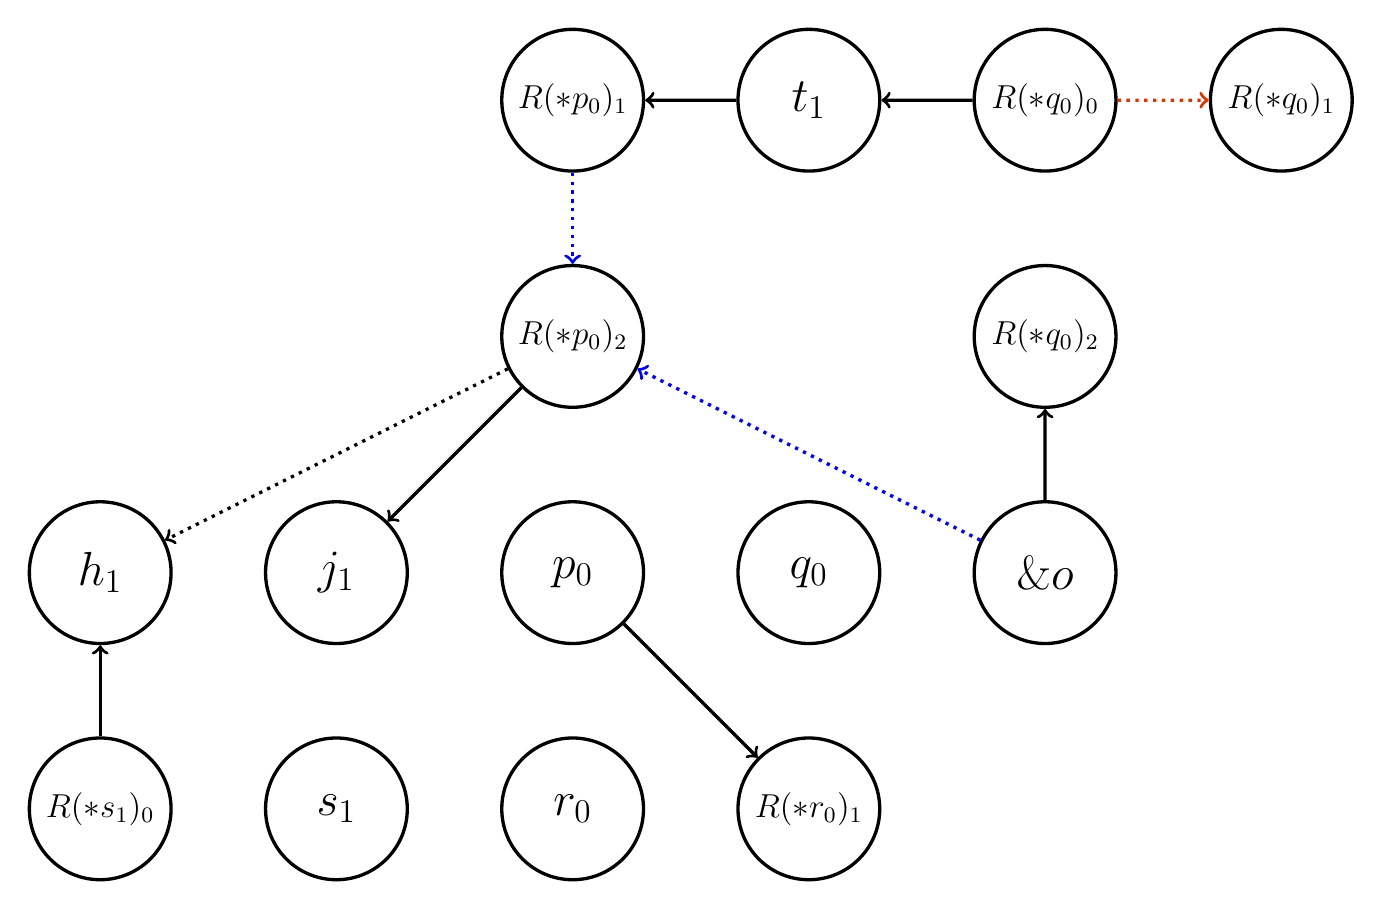
\begin{tikzpicture}[scale=3]
	\tikzstyle{every node}=[circle,draw,minimum size=1.8cm,very thick,font=\LARGE]
	\node (h1) at (-1,0) {$h_1$};
	\node (j) at (0,0) {$j_1$};
	\node (p) at (1,0) {$p_0$};
	\node (q) at (2,0) {$q_0$};
	\node (o) at (3,0) {$\&o$};
	\node (r) at (1,-1) {$r_0$};
	\node (*r01) at (2,-1) {};
	\node[draw=none,font=\large] () at (2,-1) {$R(*r_0)_1$};
	\node (s1) at (0,-1) {$s_1$};
	\node (*s10) at (-1,-1) {};
	\node[draw=none,font=\large] () at (-1,-1) {$R(*s_1)_0$};
	\node (*p02) at (1,1) {};
	\node[draw=none,font=\large] () at (1,1) {$R(*p_0)_2$};
	\node (*p01) at (1,2) {};
	\node[draw=none,font=\large] () at (1,2) {$R(*p_0)_1$};
    \node (t) at (2,2) {$t_1$};
	\node (*q00) at (3,2) {};
	\node[draw=none,font=\large] () at (3,2) {$R(*q_0)_0$};
	\node (*q01) at (4,2) {};
	\node[draw=none,font=\large] () at (4,2) {$R(*q_0)_1$};
	\node (*q02) at (3,1) {};
	\node[draw=none,font=\large] () at (3,1) {$R(*q_0)_2$};
	\draw[->,very thick] (*s10) -- (h1);
	\draw[->,very thick] (p) -- (*r01);
	\draw[->,very thick] (*q00) -- (t);
	\draw[->,very thick] (t) -- (*p01);
	\draw[->,very thick] (*p02) -- (j);
	\draw[->,very thick] (o) -- (*q02);
	\draw[dotted,red,->,very thick] (*q00) -- (*q01);
	\draw[dotted,blue,->,very thick] (*p01) -- (*p02);
	\draw[dotted,blue,->,very thick] (o) -- (*p02);
	\draw[dotted,->,very thick] (*p02) -- (h1);
	\end{tikzpicture}
    }
\end{center}
\caption{Solved constraint graph with region-based strong update}
\label{fig:RSCG}
\end{figure}

\begin{figure}[t]
\begin{center}
\begin{lstlisting}
int *out, *con, **tp, *tr;
void main()
{
  int high, low, in;
  int *hp, *lp, *ip;
  int **mem, **input;
  hp = &high, lp = &low, ip = &in;
  if (in>THRESHOLD) mem = &hp;
  else              mem = &lp;
  input = &ip, tp = &tr;
  copy(mem, input);
  mem = &hp;
  copy(input, mem);
}

void copy(int **p, int **q)
{
  int *tmp = *q;
  *p = tmp;
  out = *p;
  *tp = p;
  con = *tr;
}
\end{lstlisting}
\end{center}
\caption{Motivation example}
\label{fig:example}
\end{figure}

\begin{table}[h]
%\begin{tabular}{|p{0.16\paperwidth}|p{0.45\paperwidth}|}
\begin{tabular}{|rcl|l|}
\hline
    $t_1$ & = & $*q_0$; & $\ptrmap{t_1} = \{(g,C_1,may),(l,C_2,may)\}$\\
	$*p_0$ & = & $t_1$; & $\ptrmap{x_1} = \{(m,C_1,may),(g,C_1,may)\}$\\
     & & & $\ptrmap{y_1} = \{(n,C_1,may),(g,C_1,may)\}$\\
     & & & $\ptrmap{z_1} = \{(l,C_2,may)\}$\\
	$*q_0$ & = & malloc(4); & $\ptrmap{h_1} = \{(g,C_1,may),(o,C_1,may)\}$\\
     & & & $\ptrmap{z_2} = \{(l,C_2,may),(o,C_2,may)\}$\\
	$j_1$ & = & $*p_0$; & $\ptrmap{j_1} = \{(m,C_1,may),(n,C_1,may),(l,C_2,may),(g,C_1,may)\}$\\
	$*r_0$ & = & $p_0$; & $\ptrmap{s_1} = \{(x,C_1,may),(y,C_1,may),(z,C_2,may)\}$\\
	$h_1$ & = & $*s_1$; & $\ptrmap{h_2} = \{(m,C_1,may),(n,C_1,may),(l,C_2,may),(g,C_1,may)\}$\\
\hline
    $t_1$ & = & $R(*q_0)_0$; & $\ptrmap{t_1} = \{(g,C_1,M),(l,C_2,M)\}$\\
    $R(*p_0)_1$ & = & $t_1$; & $\ptrmap{R(*p_0)_1} = \{(g,C_1,M),(l,C_2,M)\}$\\
	$R(*q_0)_1$ & = & malloc(4); & $\ptrmap{R(*q_0)_1} = \{(o,T,M)\}$\\
	$j_1$ & = & $R(*p_0)_1$; & $\ptrmap{j_1} = \{(g,C_1,M),(l,C_2,M)\}$\\
	$R(*r_0)_1$ & = & $p_0$; & $\ptrmap{R(*r_0)_1} = \{(x,C_1,M),(y,C_1,M),(z,C_2,M)\}$\\
    $\bm{s_1}$ & \textbf{=} & $\bm{\chi(s_0)}$ & $\ptrmap{s_1} = \{(x,C_1,M),(y,C_1,M),(z,C_2,M)\}$\\
    $h_1$ & = &$R(*s_1)_1$; & $\ptrmap{h_1} = \{(g,C_1,M),(l,C_2,M)\}$\\
\hline
\end{tabular}
\end{table}

Since this is a context-sensitive analysis, there should be some guard conditions on the copy edges so that the value of $z_0$ will not be propagated into $x_1$ and $y_1$. Also the value of $h_0$ cannot flow into $z_1$. Here we just omit these conditions. $*q_0 = malloc(4)$ will allocate a new heap object $o$ and assign the address of $o$ to the variables pointed to by $q_0$. Because $q_0$ has two points-to targets, $h$ and $z$, both of them can only perform weak updates here, which means their new value will keep the original ones and $\&o$. These constraints are illustrated by blue dotted lines. The load statement $j_1 = *p_0$ will introduce new copy edges between $j$ and $p_0$'s points-to targets: $x$, $y$ and $z$ which are red lines in the graph. In this program, $r$ will always point to a singleton: $s$ under every context condition. So $*r_0 = p_0$ will strong updates $s$'s value with $p_0$'s. The last store constraint from $s_1$ to $h_2$ will have the same effect as $j_1 = *p_0$ as $s_1$ is equal to $p_0$ after the previous strong updates. The final points-to map after analyzing function $foo$ is shown in figure~\ref{fig:comparison}(d). Due to the may points-to relations from $p$ to $x$ and $y$, both $j_1$ and $h_1$ will have the original value of $x$ and $y$.

After a fast pre-analysis, all the expressions existed in the program will be assigned to a level according to the points-to relations of the memory locations they may represent. For example, $*p$, $*s$, x and y will be assigned level 1. To guarantee the correctness of memory SSA form, Low-level region's points-to information will not be computed unless all the higher level regions' are done. In our motivation example, there're four level groups: $\{c,r\}$, $\{a,b,p,q,s,*r\}$, $\{h,x,y,z,j,t,*p,*q,*s\}$, $\{m,n,l,g\}$.

The final constraint graph computed by our region-based strong updates analysis is shown in figure~\ref{fig:CG}(c). As we consider every expression as a region, we can use $R(*p_0)$, $R(*q_0)$, $R(*r_0)$ and $R(*s_1)$ to represent the expressions $*p_0$, $*q_0$, $*r_0$ and $*s_1$. Compared with figure~\ref{fig:CG}(b), initially there're only five copy constraints between region variables in the graph. During the analysis, we may find that Considering region aliases, when $RP$ is being modified, $RQ$ may also be modified under some context conditions.
